\documentclass[a4paper,11pt]{article}

\title{Statistical Inference of Discretely Observed Compound Poisson Processes and Related Jump Processes}
\author{Suraj Shah}

\usepackage{amsmath}
\usepackage{amssymb}
\usepackage{amsfonts}
\usepackage{bbm}

\usepackage{amsthm}
\usepackage{cleveref}

\usepackage{relsize}

\usepackage{graphicx}
\graphicspath{ {./plots/} }

%code below for biblography environments
\usepackage[numbers]{natbib} 
\bibliographystyle{plainnat} 
\usepackage{cite}
\usepackage{url}

\theoremstyle{theorem}
\newtheorem{thm}{Theorem}
\newtheorem{lem}{Lemma}[section]
\crefname{lem}{Lemma}{Lemmas}
\newtheorem{prop}{Proposition}[section]
\newtheorem*{trapezoid}{Trapezoid Rule}
\newtheorem*{fft}{Fast Fourier Transform}

\theoremstyle{definition}
\newtheorem{defn}{Definition}[section]
\newtheorem*{eg}{Example}

\theoremstyle{remark}
\newtheorem*{rem}{Remark}
\newtheorem*{note}{Note}
\newtheorem{case}{Case}

\providecommand{\E}{\mathbb{E}}

\begin{document}

\maketitle

\begin{abstract}
Jump processes are a group of continuous-time stochastic processes whose values move in discrete amounts at random times. The compound Poisson process sits near the centre of this rich class of processes, and its versatility makes it an exceptional candidate for modelling phenomena in the world. However, its versatility comes at a price - statistical inference on them is difficult when we only observe values at discrete points in time because a significant amount of information is lost. 

In this essay, we discuss and implement various nonparametric methods for the estimation of a compound Poisson processes' defining properties. In particular, we first employ a spectral approach using suitable kernel functions as shown in van Es et al. \citep{vanes2007} and in Comte et al. \citep{comte2014}. We then visit nonparametric Bayesian inference and show its use following the approach laid out in Gugushvili et al. \citep{gugushvili2018}. Finally, we construct a novel Bayesian procedure based on an overlooked result in Duval \citep{duval2013} and illustrate its performance via numerical simulations.

Since this essay is computational in flavour, we focus mainly on carefully deriving the forms of the estimators and analyse their performance on various example simulations. Therefore, we omit many theoretical guarantees of these estimators, but such results exist and are abundant in the literature referenced. 
\end{abstract}

\pagebreak

\tableofcontents

\pagebreak

\section{Introduction}

Consider an established social media company, e.g. Facebook, with a database server handling read and write requests for photos. Users may upload or delete a photo, and such events occur at random. Also, their photos are of varying size due to factors such as camera quality or cropping, and, since we have little knowledge of these factors, we may assume that the amount of data required to store each photo is random. 

An Engineer may ask questions like 'Is the capacity of the database server enough to store the photos?' or 'What is the amount of traffic on the server in a given time period?'. Under normal conditions, we can model the amount of data in the database server at a given time as a compound Poisson process and, due to the high frequency of writes, we may only be able to know this amount at discrete points in time. Thus, statistical inference on these discrete observations may be of great interest to gain more insight into such questions.   

We begin by providing intuition behind the compound Poisson process and look at some of its key properties. We then formulate the statistical inverse problem at hand and address necessary technical details to set up the basic framework for estimation.

\subsection{Compound Poisson Processes}

Compound Poisson processes push the boundaries of Poisson processes, by allowing the jump sizes to follow a distribution rather than being of fixed unit size. We associate compound Poisson processes with the following three key properties:
\begin{enumerate}
\item The occurrence of the jumps follow a Poisson process,
\item The jumps sizes are independent, and follow a common distribution,
\item The interarrival times between the jumps and the sizes of the jumps are mutually independent random variables.
\end{enumerate}

\begin{defn}[Poisson Process]
A \textit{Poisson process with intensity $\lambda$} is a non-negative, non-decreasing, integer-valued stochastic process $(N_{t})_{t \geq 0}$ starting at 0 with the following properties:

\begin{enumerate}

\item It has independent increments:

For every $n \in \mathbb{N}$ and $t_1, \dotsc, t_n$ such that $0 \leq t_{1} \leq t_{2} \leq \dotsb \leq t_{n}$, we have that 
\[
N_{t_{n}} - N_{t_{n-1}}, \dotsc , N_{t_2} - N_{t_1}, N_{t_{1}}
\]
are mutually independent,
\item The number of occurrences in any interval of length $\Delta$ is a Poisson random variable with parameter $\lambda \Delta$:

For every $\Delta > 0$ and $t \geq 0$ we have that
\[ 
N_{(t+1) \Delta} - N_{t \Delta} \sim {\rm Po}(\lambda \Delta).
\]
\end{enumerate}
\end{defn}

We use the well-known property that a Poisson process with intensity $\lambda$ has $\exp(\lambda)$-distributed inter-arrival times to simulate the Poisson process.

\begin{figure}[h!]
\centering
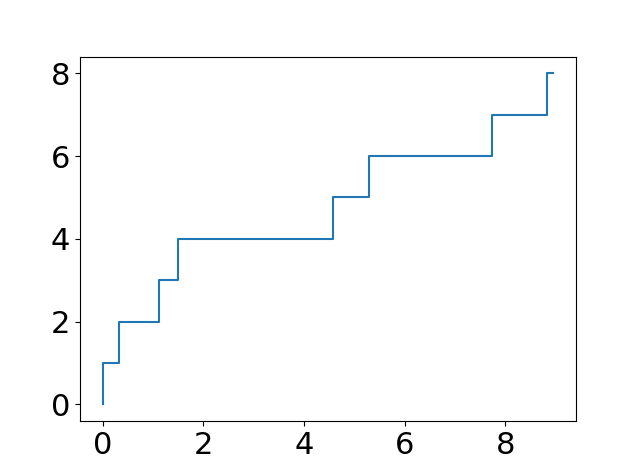
\includegraphics[scale=0.5]{poisprocess.png}
\caption{Simulation of a Poisson process with intensity 1}
\label{poisprocess}
\end{figure}

As we can see in Figure \ref{poisprocess}, the jump sizes are of unit length. The compound Poisson process extends this by allowing the jumps to vary in size.

\begin{defn}[Compound Poisson Process]
Let $(N_{t})_{t \geq 0}$ be a Poisson process with intensity $\lambda$. Let $Y_{1}, Y_{2}, \dotsc$ be a sequence of i.i.d random variables with common distribution $F$. Also assume that this sequence is independent of the Poisson process.

Then, a \textit{compound Poisson process with intensity $\lambda$ and jump distribution $F$} is a stochastic process $(X_{t})_{t \geq 0}$ such that
\[
X_{t} = \sum_{i=1}^{N_t} Y_{i}
\]
By convention, we take $X_t = 0$ if $N_t = 0$.
\end{defn}

\begin{figure}[h]
\centering
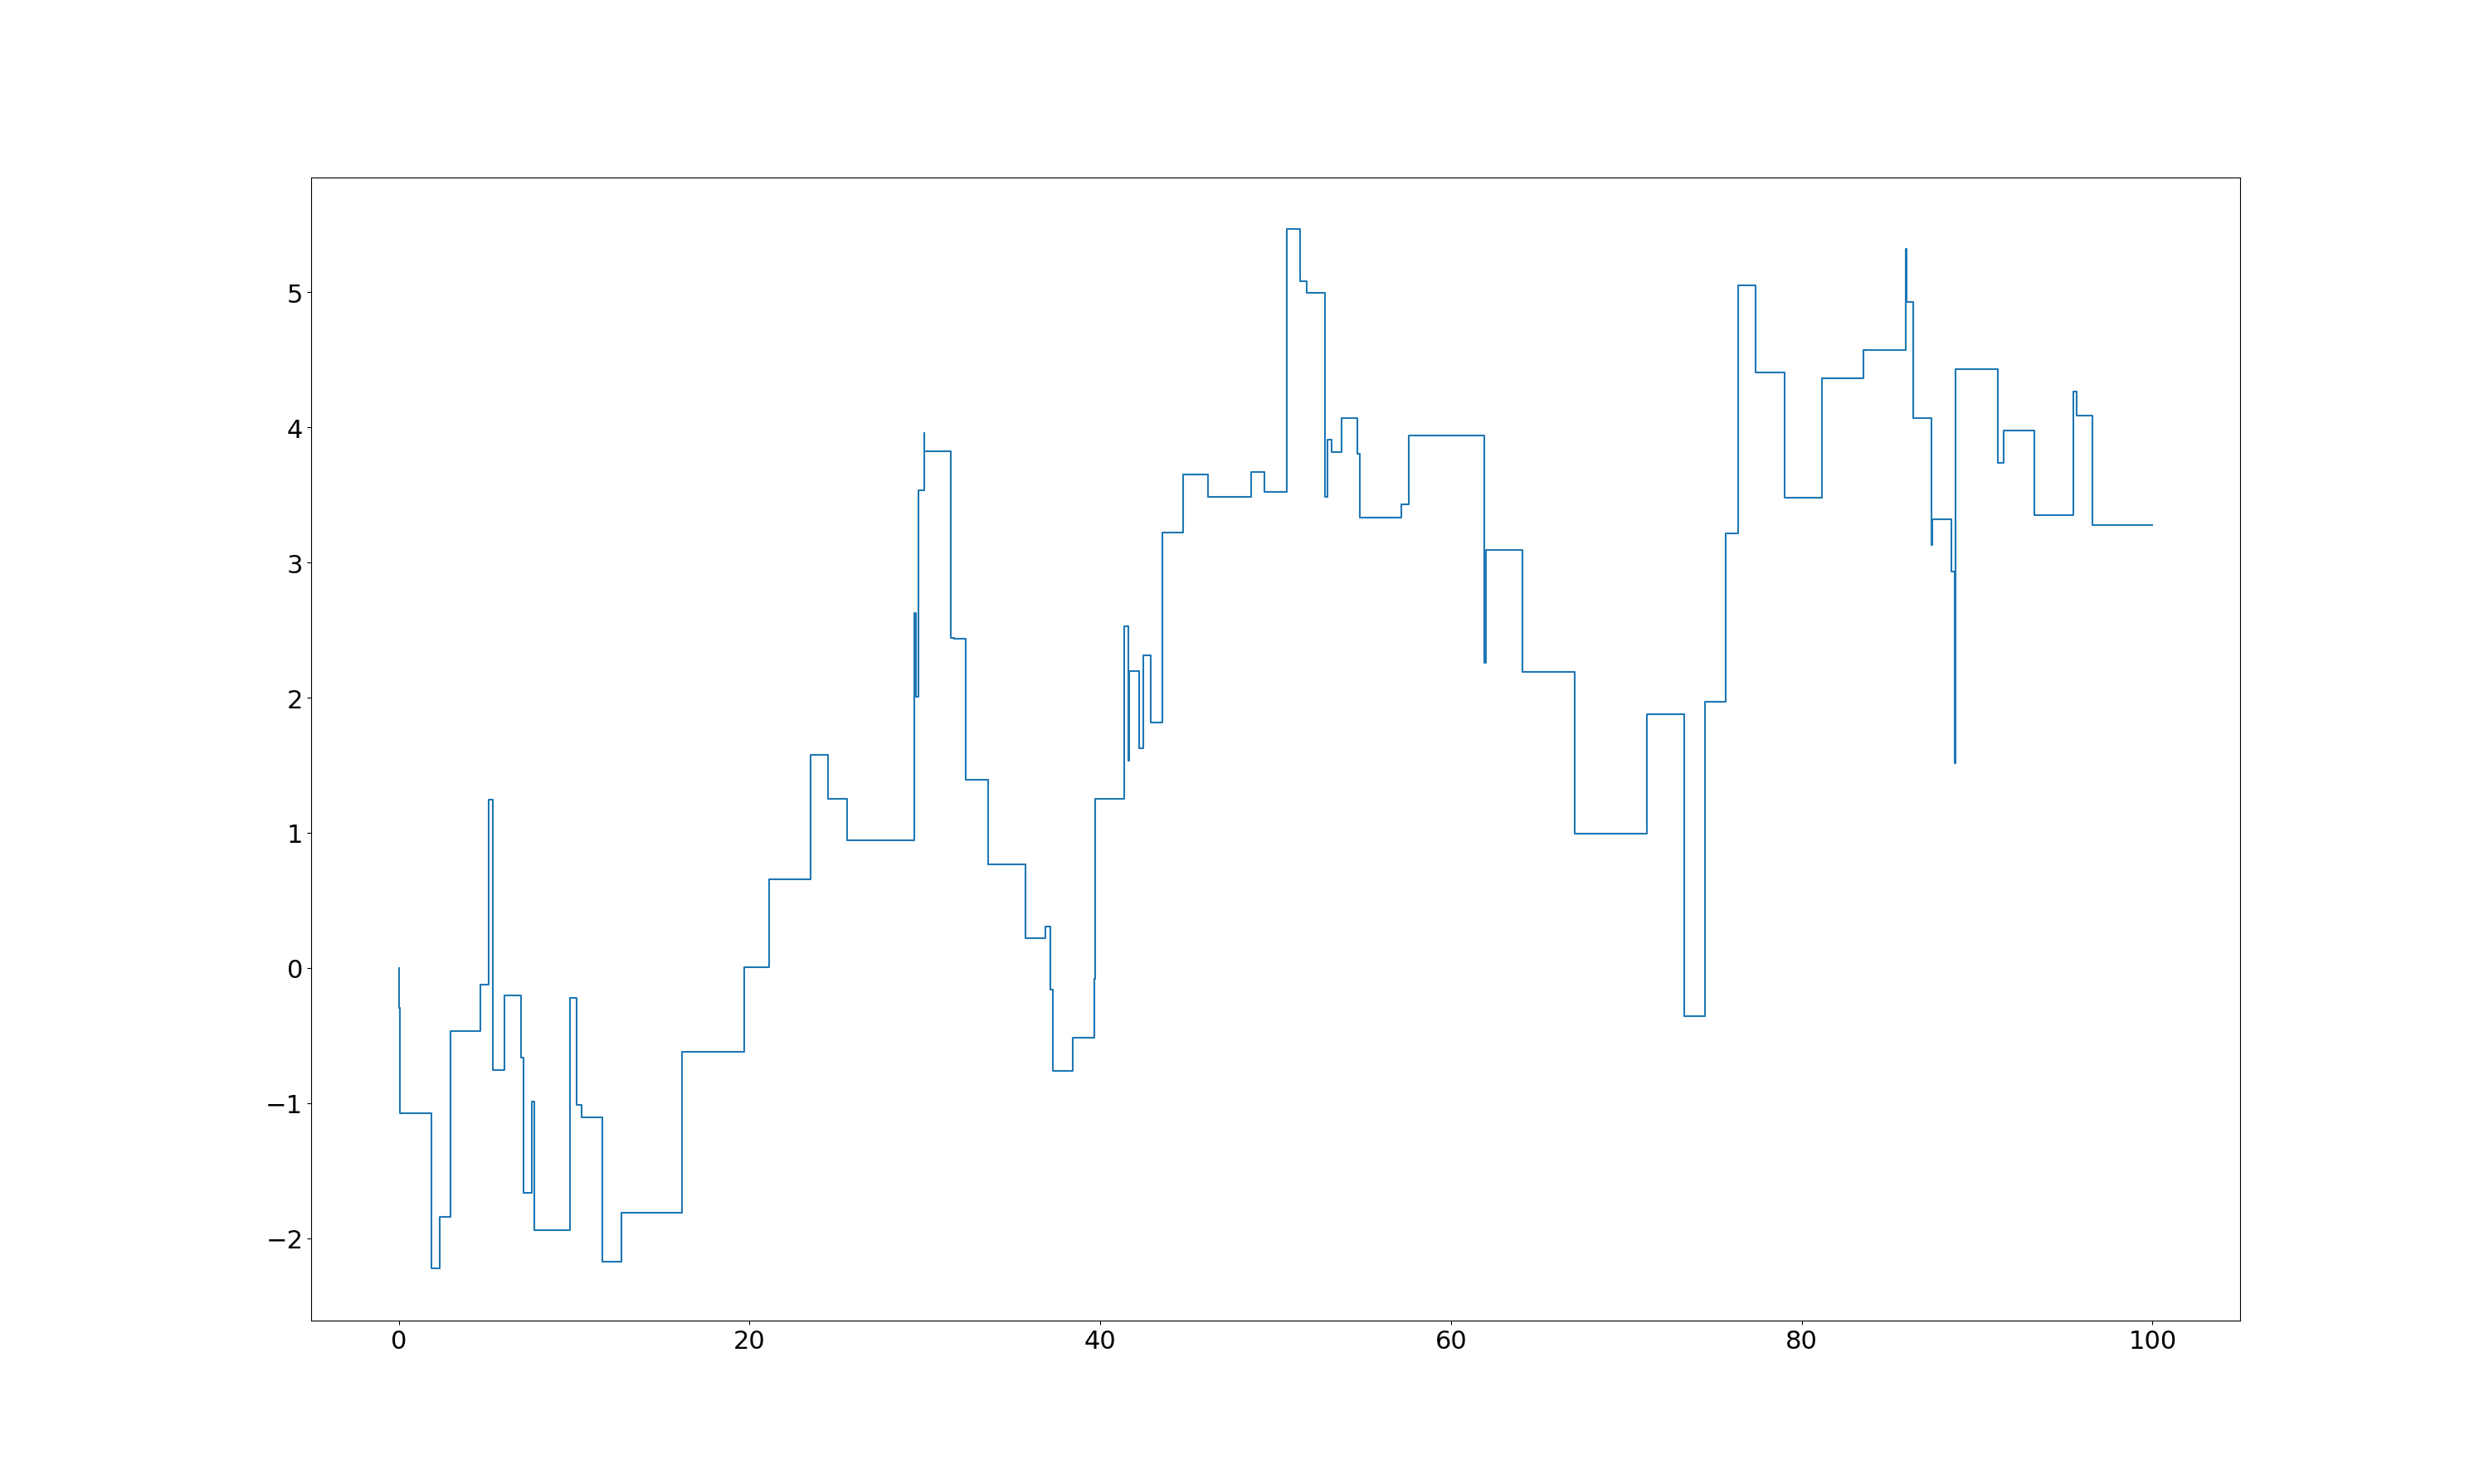
\includegraphics[scale=0.1]{cppsim.png}
\caption{Simulation of a compound Poisson process with intensity 1 and jump distribution $\mathcal{N}(0,1)$}
\label{cppsim}
\end{figure}

\subsection{The Statistical Non-Linear Inverse Problem}

In our example, we can only observe the process up to some time $T$. In addition, we can only observe the process at a discrete set of points in time, say every second. In other words we obtain observations $X_{\Delta}, X_{2\Delta}, \dotsc, X_{n\Delta}$ for some fixed $\Delta > 0$ and $n := \left\lfloor \frac{T}{\Delta} \right\rfloor$. We also assume that the intensity $\lambda$ of the compound Poisson process is known and that the jump distribution $F$ has jump density $f$. In this essay, we want to recover the jump density $f$ of the $Y_i$ jumps in the compound Poisson process from these $n$ observations.

By the second property of a Poisson process and the i.i.d assumption of the jump distribution we get that for $0 < i \leq n$ and $X_{i\Delta} \neq X_{(i-1)\Delta}$
\[
X_{i\Delta} - X_{(i-1)\Delta} = \sum_{j=N_{(i-1)\Delta} + 1}^{N_{i\Delta}}{Y_j} 
=^{d} \mathlarger{\mathlarger{\sum}_{j=1}^{N_{i\Delta} - N_{(i-1)\Delta}}{Y_j}} =^{d} \sum_{j=1}^{N}{Y_j}
\]
where $N \sim \mathrm{Po}(\lambda\Delta)$. By the first property of Poisson processes, all such $Z_i := X_{i\Delta} - X_{(i-1)\Delta}$ are mutually independent. Thus it is much easier to convert our observations into this form, and we call each observation increment $Z_i = \sum_{j=1}^{N}{Y_j}$ a \textit{Poisson random sum with parameter $\lambda \Delta$}.  

\begin{rem}
We shall see in Proposition ?? that an observation increment $Z_i$ of zero provides no additional information on the jump size density. Therefore, we focus on the non-zero increments and assume that we sample up to some random time $T_n$, where $T_n$ is the first moment we get $n$ non-zero increment observations.
\end{rem}

\subsection{Properties of Poisson random sums}

We have now converted our problem into the problem of estimating the jump size density $f$ from $n$ observations of non-zero independent increments $(Z_i)_{i \geq 0})$. Each of the $Z_i$ are Poisson random sums with parameter $\lambda \Delta$, and thus we state and prove some properties of Poisson random sums that we will use throughout the essay.

\begin{prop} \label{characteristicPS}
For Poisson random sum $Z$ with parameter $\lambda \Delta$, the characteristic function of $X$, denoted by $\phi_{Z}$, is given by 
\[
\phi_Z(t) = \mathbb{E}e^{itZ} = e^{-\lambda\Delta + \lambda\Delta\phi_{f}(t)}
\]
where $\phi_{f}$ denotes the characteristic function of one of its terms $Y$ with density $f$. 
\end{prop}

\begin{rem}
We will often, for convenience sake, denote $\phi_{X}$ to be the characteristic function of a random variable $X$ as well as $\phi_{g}$ to be the characteristic function of a random variable $X$ with density $g$. To avoid confusion, all densities will be written using a lower-case symbol, whilst random variables will be written using an upper-case symbol. 
\end{rem}

\begin{proof}
\begin{align*}
\phi_{Z}(t) &= \E e^{itZ} = \E e^{it\sum_{i=1}^{N}{Y_{i}}} 
= \E \prod_{i=1}^{N}{e^{itY_{i}}} 
= \E \left[ \E \left[ \prod_{i=1}^{N}{e^{itY_{i}}} \middle| N \right] \right] \\
          &= \E \prod_{i=1}^{N}{\E \left[ e^{itY_{1}} \middle| N \right]} & \text{(by i.i.d assumption of the } Y_{i}\text{'s)}  \\
          &= \E \left[ \prod_{i=1}^{N(\lambda)}{\phi_{f}(t)} \right] & \text{(}Y_{1} \text{ and } N(\lambda) \text{ are independent)} \\
          &= \E \left[ \exp(N(\lambda) \ln\phi_{f}(t)) \right] \\
          &= \exp(\lambda(e^{\ln\phi_{f}(t)} - 1)) & \text{(MGF of a Poisson random variable)} \\
          &= e^{-\lambda + \lambda \phi_{f}(t)}
\end{align*}
\end{proof}

\begin{prop}
The distribution of the Poisson random sum $X = \sum_{i=1}^{N}{Y_i}$ where $Y_i \overset{\text{i.i.d}}{\sim} F$ and $N \sim \text{Po}(\lambda)$ is absolutely continuous with respect to measure $\mu = \delta_{\{0\}} + \mathrm{Leb}$ and has Radon-Nikodym derivative
\begin{equation} \label{R-N duval}
\frac{\mathrm{d}\mathbb{P}_{X}}{\mathrm{d}\mu}(x) = e^{-\lambda \Delta} \mathbbm{1}_{\{0\}}(x) + (1 - e^{-\lambda \Delta})\sum_{m=1}^{\infty}{a_m(\lambda \Delta) f^{\ast m}(x)\mathbbm{1}_{\mathbb{R}\setminus \{0\}}(x)}
\end{equation}
where
\begin{equation}
a_m(\lambda \Delta) = \frac{1}{e^{\lambda \Delta} - 1}\frac{(\lambda \Delta)^m}{m!}
\end{equation}
and $f*m$ denotes the m-fold convolution of $f$ with itself.
\end{prop}

\begin{proof}
Suppose we have $A \in \mathcal{B}$ such that $\mu(A) = 0$. Then $0 \notin A$ and $A$ has Lebesgue-measure zero. Therefore, under event $A$, the Poisson random sum $X$ is non-zero and we have 
\begin{align*}
\mathbb{P}_{X}(A) &= \sum_{n=1}^{\infty}{\mathbb{P}(Y_1 + \dotsb + Y_n  \in A, N = n)} \\
&= \sum_{n=1}^{\infty}{\mathbb{P}(Y_1 + \dotsb + Y_n  \in A)\mathbb{P}(N = n)} \\
&= 0
\end{align*}
since $Y_1 + \dotsb + Y_n$ has a density. Therefore, the first statement follows. Note that for $A \in \mathcal{B}$
\begin{align*}
\mathbb{P}_{X}(A) &= \mathbb{P}(N = 0)\int_{A}{d\delta_{\{0\}}} + \sum_{n=1}^{\infty}{\mathbb{P}(Y_1 + \dotsb + Y_n  \in A)\mathbb{P}(N = n)} \\
&= e^{\lambda \Delta}\int_{A}{d\delta_{\{0\}}} + (1 - e^{\lambda \Delta})\sum_{n=1}^{\infty}{a_m(\lambda \Delta)\int_{A}{f^{\ast m}(x)dx}} & \text{Using Lemma \ref{conv}} \\
&= \int_{A}\left[{e^{\lambda \Delta} \mathbbm{1}_{\{0\}}(x) + (1 - e^{\lambda \Delta})\sum_{m=1}^{\infty}{a_m(\lambda \Delta) f^{\ast m}(x)\mathbbm{1}_{\mathbb{R}\setminus \{0\}}(x)}}\right]d\mu(x)
\end{align*}
\end{proof}

\section{Spectral Approach}

Now we have formulated the problem, we visit some methods for estimating the unknown density $f$. Since adding a Poisson number of $Y$'s is referred to as compounding, much of the literature refers to the problem of recovering density $f$ of $Y$'s from observations of $X$ as decompounding.

The approach of decompounding was famously proposed by Buchmann and Gr\"{u}bel to estimate the density $f$ for discrete and continuous cases of the distribution $F$ of the $Y$'s.

Van Es built on this idea for fixed sampling rate $\Delta = 1$ using the L\'{e}vy - Khintchine formula. We explain the idea behind this method and show its strength through various examples.

\subsection{Van Es}

\subsubsection{Construction of Density Estimator via suitable inversion of characteristic functions}

We first note the following property:

We can rewrite $\phi_{X}(t)$ as:

\begin{align}
\phi_{X}(t) &= e^{-\lambda}(e^{\lambda \phi_{f}(t)} - 1 + 1) \nonumber \\
		    &= e^{-\lambda} + e^{-\lambda}(e^{\lambda \phi_{f}(t)} - 1) \nonumber \\
		    &= e^{-\lambda} + e^{-\lambda}\frac{e^{\lambda} - 1}{e^{\lambda} - 1}(e^{\lambda \phi_{f}(t)} - 1) \nonumber \\
		    &= e^{-\lambda} + \frac{1 - e^{-\lambda}}{e^{\lambda} - 1}(e^{\lambda \phi_{f}(t)} - 1) \label{eq:charX}
\end{align}

Since a zero jump size provides no additional information on the density $f$, we want to gain information about $X$ conditional on the event that there is at least one jump. Seeing that $X \;|\; N(\lambda) > 0$ has a density is somewhat intuitive, but we provide a proof of this.

\begin{lem}
The random variable $X \;|\; N(\lambda) > 0$ has a density.
\end{lem}
\begin{proof}
By the Radon-Nikodym Theorem, a random variable $X$ has a density if and only if $\mathbb{P}(X \in A) = 0$ for every Borel set $A$ with Lebesgue measure zero.

Suppose that Leb$(A) = 0$. Then
\begin{align*}
\mathbb{P}(X \in A | N(\lambda) > 0)
&= \frac{1}{\mathbb{P}(N(\lambda) > 0)}\sum_{n=1}^{\infty}{\mathbb{P}\left(Y_{1} + \dotsb + Y_{n} \in A, N(\lambda) = n\right)} \\
&= \frac{1}{\mathbb{P}(N(\lambda) > 0)}\sum_{n=1}^{\infty}{\mathbb{P}\left(Y_{1} + \dotsb + Y_{n} \in A\right) \mathbb{P}(N(\lambda) = n)}                                     
\end{align*}
Note that for each $n, Y_{1} + \dotsb + Y_{n}$ has a density so $\mathbb{P}\left(Y_{1} + \dotsb + Y_{n} \in A\right) = 0$. Thus the result follows.

\end{proof}
Let $g$ be the density of $X \;|\; N(\lambda) > 0$. 

Let $\phi_{g}(t) = \E \left[ e^{itX} \;\middle|\; N(\lambda) > 0 \right] = \frac{\E \left[ e^{itX} \mathbbm{1}(N(\lambda) > 0) \right]}{\mathbb{P}(N(\lambda) > 0)}$.

Then
\begin{align*}
\phi_{X}(t) &= \E \left[ e^{itX} \mathbbm{1}(N(\lambda) = 0) \right] + \E \left[ e^{itX} \mathbbm{1}(N(\lambda) > 0) \right] \\
            &= \mathbb{P}(N(\lambda) = 0) + \mathbb{P}(N(\lambda) > 0) \phi_{g}(t) \\
            &= e^{-\lambda} + (1 - e^{-\lambda})\phi_{g}(t)
\end{align*}

Therefore, using (\ref{eq:charX}), we get that
\begin{equation}
\phi_{g}(t) = \frac{1}{e^{\lambda} - 1}(e^{\lambda \phi_{f}(t)} - 1) \label{eq:charg}
\end{equation}

Thus, we can see from this that if we were to obtain an estimator for $\phi_{g}(t)$, then by suitable inversion of the formula in (\ref{eq:charg}), we would obtain an estimator for $\phi_{f}(t)$.

In order to rewrite (\ref{eq:charg}) in terms of $\phi_{f}(t)$, we must be able to invert the complex exponential function since $\phi_{f}(t)$ takes complex values. However, such function is not invertible since it is not bijective: in particular it is not injective as $e^{w + 2 \pi i} = e^{w} \ \forall w \in \mathbb{C}$.

Therefore, we use the following lemmas concerning the distinguished logarithm:

\begin{lem} \label{lma1}
If $h_{1} : \mathbb{R} \to \mathbb{C}$ and $h_{2} : \mathbb{R} \to \mathbb{C}$ are continuous functions such that $h_{1}(0) = h_{2}(0) = 0$ and $e^{h_{1}} = e^{h_{2}}$, then $h_{1} = h_{2}$. 
\end{lem}

\begin{proof}
See Appendix.
\end{proof}

\begin{lem} \label{lma2}
If $\phi : \mathbb{R} \to \mathbb{C}$ is a continuous function such that $\phi(0) = 1$ and $\phi_{g}(t) \neq 0 \ \forall t \in \mathbb{R}$ then there exists a unique continuous function $h : \mathbb{R} \to \mathbb{C}$ with $h(0) = 0$ and $\phi(t) = e^{h(t)}$ for $t \in \mathbb{R}$. 
\end{lem}

\begin{proof}
See Appendix.
\end{proof}

Therefore, for such a function $\phi$ as described in the Lemma, we say that the unique function $h$ is the distinguished logarithm and we denote $h(t) = \text{Log}(\phi(t))$. Note also that for $\phi$ and $\psi$ satisfying the assumptions of the Lemma, we have $\text{Log}(\phi(t)\psi(t)) = \text{Log}(\phi(t)) + \text{Log}(\psi(t))$ as expected.  

Therefore, noting that $\phi(t) = e^{\lambda(\phi_{f}(t) - 1)}$ is a continuous function satisfying $\phi(0) = 1$ and $\phi(t) \neq 0 \ \forall t \in R$, we get that
\begin{align*}
\lambda(\phi_{f}(t) - 1) &= \text{Log}\left(e^{\lambda (\phi_{f}(t) - 1)}\right)& \text{(\cref{lma1})} \\
                         &= \text{Log}\left(e^{-\lambda}\left[(e^{\lambda} - 1)\phi_{g}(t) + 1\right] \right) \\
                         &= -\lambda + \text{Log}\left((e^{\lambda} - 1)\phi_{g}(t) + 1\right)
\end{align*}

Therefore,
\begin{equation} \label{eq:charf}
\phi_{f}(t) = \frac{1}{\lambda}\text{Log}\left((e^{\lambda} - 1)\phi_{g}(t) + 1\right)
\end{equation} 

By Fourier inversion, for integrable $\phi_{f}$ we have
\begin{equation} \label{eq:fourier}
f(x) = \frac{1}{2\pi\lambda}\int_{-\infty}^{\infty}{e^{-itx}\text{Log}\left((e^{\lambda} - 1)\phi_{g}(t) + 1\right)}dt
\end{equation}

This suggests that if we can estimate $\phi_{g}(t)$, then we have an estimate of $f$.

\subsubsection{Kernel density estimators}

We provide the intuition behind choosing our estimator for $g$ on observations of non-zero jump size as a kernel density estimator.

Let $X$ be a random variable with probability density $p$ with respect to the Lebesgue measure on $\mathbb{R}$. The corresponding distribution function is $F(x) = \int_{-\infty}^{x}{p(t)}dt$.

Consider n i.i.d observations $X_{1}, \dotsc , X_{n}$ with same distribution as $X$. The empirical distribution function is given by 
\[
F_{n}(x) = \frac{1}{n}\sum_{i=1}^{n}{I(X_{i} \leq x)}
\]  

By the Strong Law of Large Numbers, since for fixed $x$, $I(X_{i} \leq x)$ are i.i.d , we have that
\[
F_{n}(x) \to \E \left[ I(X_{1} \leq x) \right] = \mathbb{P}(X \leq x) = F(x)
\]
almost surely as $n \to \infty$.

Therefore, $F_{n}(x)$ is a consistent estimator of $F(x)$ for every $x \in \mathbb{R}$. Also note that $p(x) = \frac{\mathrm{d}}{\mathrm{d}x}F(x)$, so for sufficiently small $h > 0$ we can write an approximation
\[
p(x) \approx \frac{F(x+h) - F(x-h)}{2h}
\]
Thus, intuitively we can replace $F$ by our empirical distribution function $F_{n}$ to give us an estimator $\hat{p}_{n}(x)$ of $p(x)$
\begin{align*}
\hat{p}_{n}(x) &= \frac{F_{n}(x+h) - F_{n}(x-h)}{2h} \\
               &= \frac{1}{2nh}\sum_{i=1}^{n}{I(x - h < X_{i} \leq x + h)} \\
               &= \frac{1}{nh}\sum_{i=1}^{n}{K_{0}\left(\frac{x - X_{i}}{h}\right)}
\end{align*}
where $K_{0}(u) = \frac{1}{2}I(-1 < u \leq 1)$.

A simple generalisation is to replace $K_{0}$ by some arbitrary (but well-chosen) integrable function $K : \mathbb{R} \to \mathbb{R}$ such that $\int{K(u)}du = 1$ and $K(u) = K(-u)$ for every $u \in \mathbb{R}$. Such a function $K$ is called a \textit{kernel} and the parameter $h$ is called a \textit{bandwidth} of the estimator
\begin{equation} \label{kde}
\hat{p}_{n}(x) = \frac{1}{nh}\sum_{i=1}^{n}{K\left(\frac{x - X_{i}}{h}\right)}
\end{equation}
We call this estimator a \textit{kernel density estimator}.

Thus, for some kernel $w$ with characteristic function $\phi_{w}$ and observations $Z_{1}, \dotsc , Z_{n}$, we estimate density $g$ by the kernel density estimator
\[
g_{nh}(x) = \frac{1}{nh}\sum_{i=1}^{n}{w\left(\frac{x - Z_{i}}{h}\right)}
\]
Letting $\phi_{\text{emp}}(t) = \frac{1}{n}\sum_{j=1}^{n}{e^{itZ_{j}}}$ be the empirical characteristic function, we get that
\begin{align*} \label{charformula}
\phi_{g_{nh}}(t) &= \int_{-\infty}^{\infty}{e^{itx}g_{nh}(x)}dx \\
                 &= \int_{-\infty}^{\infty}{e^{itx}\frac{1}{nh}\sum_{j=1}^{n}{w\left(\frac{x - Z_{j}}{h}\right)}}dx \\
                 &= \frac{1}{n}\sum_{j=1}^{n}{e^{itZ_{j}}}\int_{-\infty}^{\infty}{e^{ithy}w(y)}dy &\left(\text{by the substitution } y = \frac{x - Z_{j}}{h} \right) \\
                 &= \phi_{\text{emp}}(t)\phi_{w}(ht)
\end{align*}

In view of (\ref{eq:fourier}) It is tempting to introduce an estimator $\hat{f}_{nh}$ of $f$

\begin{equation} \label{fnh}
\hat{f}_{nh}(x)= \frac{1}{2\pi\lambda}\int_{-\infty}^{\infty}{e^{-itx}\text{Log}\left((e^{\lambda} - 1)\phi_{\text{emp}}(t)\phi_{w}(ht) + 1\right)}dt
\end{equation}
but this brings two main issues:
\begin{enumerate}
\item In light of \cref{lma2}, we may have some Borel set $A$ with non-zero Lebesgue measure such that $(e^{\lambda} - 1)\phi_{\text{emp}}(t)\phi_{w}(ht) + 1$ is zero for $ t \in A$. The distinguished logarithm is undefined under such sets and thus our estimator of $f$ is undefined in this case.
\item There is no guarantee that the integral is finite. For example,
\[
\phi_{g_{nh}}(t) = \frac{\exp(e^{it}) - 1}{e^{\lambda} - 1}
\]
would give $\hat{f}_{nh}(1)$ to be infinity.
\end{enumerate}

In order to prove asymptotic properties, we must adjust our estimators by bounding $\hat{f}_{nh}$ for each $n$ using a suitable sequence $(M_{n})_{n \geq 1}$. However, for our discussion, we note such limitations and provide simulations for examples where these two cases do not occur.

\subsubsection{Simulation Results}

We note that for $\lambda < \log2$, the distinguished logarithm in (\ref{fnh}) reduces to the principal branch of the logarithm. This is the logarithm whose imaginary part lies in the interval $\left(-\pi, \pi\right]$. We also note, as written above, that bounding $\hat{f}_{nh}$ by a suitable sequence is not needed in practice. Therefore, we can use (\ref{fnh}) to compute our estimator with the principal branch of the logarithm, provided $\lambda < \log 2$.

We use the following kernel $w$ given by
\[
w(t) = \frac{48t(t^{2} - 1)\cos t - 144(2t^{2} - 5)\sin t}{\pi t^{7}}
\]

This kernel has a fairly complicated form but its characteristic function $\phi_{w}(t)$ has a much simpler expression given by
\[
\phi_{w}(t) = (1 - t^{2})^{3}\mathbbm{1}\{|t| < 1\}
\]

We can rewrite (\ref{fnh}) as $\hat{f}_{nh}(x) = \hat{f}_{nh}^{(1)}(x) + \hat{f}_{nh}^{(2)}(x)$ where

\begin{equation} \label{fnh1}
\hat{f}_{nh}^{(1)}(x) = \frac{1}{2\pi\lambda}\int_{0}^{\infty}{e^{-itx}\text{Log}\left((e^{\lambda} - 1)\phi_{\text{emp}}(t)\phi_{w}(ht) + 1\right)}dt 
\end{equation}

\begin{align}
\hat{f}_{nh}^{(2)}(x) &= \frac{1}{2\pi\lambda}\int_{-\infty}^{0}{e^{-itx}\text{Log}\left((e^{\lambda} - 1)\phi_{\text{emp}}(t)\phi_{w}(ht) + 1\right)}dt \nonumber \\
                      &= \frac{1}{2\pi\lambda}\int_{0}^{\infty}{e^{itx}\text{Log}\left((e^{\lambda} - 1)\phi_{\text{emp}}(-t)\phi_{w}(ht) + 1\right)}dt \label{fnh2}
\end{align}
since $\phi_{w}$ is symmetric.
We use a bandwidth of $0.14$. Such a bandwidth is arbitrary and we may use better methods to compute a bandwidth estimator that yields better results. This can be done via cross-validation.

We approximate (\ref{fnh1}) and (\ref{fnh2}) by the Trapezoid Rule:
 
\begin{trapezoid}
Let $\{t_{j}\}_{j=0}^{N-1}$ be a set of $N$ equally spaced values partitioning $[a,b]$, with spacing $\Delta t_{k} = \Delta t = \frac{b-a}{N}$. Then, for integrable function $f$ we get the following approximation
\begin{equation} \label{trap}
\int_{a}^{b}{f(x)dx} \approx \Delta t\left( \frac{f(t_{0}) + f(t_{N-1})}{2} + \sum_{j=1}^{N-2}{f(t_{j})}\right)
\end{equation} 
\end{trapezoid}

We can approximate (\ref{fnh1}) (and similarly (\ref{fnh2})) by computing the integrand from $0$ to some sufficiently large $M$.

We may also allow for (\ref{trap}) to be written as a 'nice' sum in order to compute the Fast Fourier Transform. Thus, we write
\begin{equation}
\int_{a}^{b}{f(t)dt} \approx \Delta t\left(\sum_{j=0}^{N-1}{f(t_{j})}\right)
\end{equation} 

Applying this to (\ref{fnh1}) and (\ref{fnh2}) we get for $t_{j} = j\eta$ for some spacing parameter $\eta$
\begin{equation}
\hat{f}_{nh}^{(1)}(x) \approx \frac{\eta}{2\pi\lambda}\sum_{k=0}^{N-1}{e^{-it_{j}x}\text{Log}\left((e^{\lambda} - 1)\phi_{\text{emp}}(t_{j})\phi_{w}(ht_{j}) + 1\right)},
\end{equation}

\begin{equation}
\hat{f}_{nh}^{(2)}(x) \approx \frac{\eta}{2\pi\lambda}\sum_{k=0}^{N-1}{e^{it_{j}x}\text{Log}\left((e^{\lambda} - 1)\phi_{\text{emp}}(-t_{j})\phi_{w}(ht_{j}) + 1\right)},
\end{equation}

We apply the Fast Fourier Transform to evaluate our functions $\hat{f}_{nh}^{(1)}$ and $\hat{f}_{nh}^{(2)}$ at points $\{x_{k}\}_{k=0}^{N-1}$.

\begin{fft}
Let $\{x_{k}\}_{k=0}^{N-1}$ be a sequence of complex numbers. The Fast Fourier Transform computes the sequence $\{Y_{j}\}_{j=0}^{N-1}$ where
\begin{equation}
Y_{j} = \sum_{k=0}^{N-1}{x_{k}e^{-ij\frac{2\pi k}{N}}}
\end{equation}
The inverse transform is given by
\begin{equation}
Y_{j} = \frac{1}{N}\sum_{k=0}^{N-1}{x_{k}e^{ij\frac{2\pi k}{N}}}
\end{equation}
\end{fft}

Thus, we employ a regular spacing with parameter $\delta$ so that our values $\{x_{k}\}_{k=0}^{N-1}$ evenly spaced and given by
\[
x_{k} = \frac{-N\delta}{2} + \delta k
\]

Thus we have
\begin{equation}
\hat{f}_{nh}^{(1)}(x_{k}) \approx \frac{1}{2\pi\lambda}\sum_{j=0}^{N-1}{e^{-ijk\eta\delta}e^{it_{j}\frac{N\delta}{2}}\psi^{(1)}(t_{j})\eta},
\end{equation}

\begin{equation}
\hat{f}_{nh}^{(2)}(x_{k}) \approx \frac{1}{2\pi\lambda}\sum_{j=0}^{N-1}{e^{ijk\eta\delta}e^{-it_{j}\frac{N\delta}{2}}\psi^{(2)}(t_{j})\eta},
\end{equation}

Therefore, we take $\eta\delta = \frac{2\pi}{N}$ and we apply FFT on the sequence $\left\lbrace e^{it_{j}\frac{N\delta}{2}}\psi^{(1)}(t_{j})\eta \right\rbrace_{j=0}^{N-1}$ to get values for $\hat{f}_{nh}^{(1)}$ and we apply IFFT on the sequence $\left\lbrace e^{-it_{j}\frac{N\delta}{2}}\psi^{(2)}(t_{j})\eta \right\rbrace_{j=0}^{N-1}$ to get values for $\hat{f}_{nh}^{(2)}$.

We take $N$ to be a power of 2 for computational speed up in calculating the Discrete Fourier Transforms and we choose $\eta$ relatively small so that $\delta$ can be relatively larger and so points are relatively separate from one another.

The results for $N = 16384$ and $\eta = 0.01$ based on 1000 observations can be shown in Figure \ref{stdNormal}.

\begin{figure}[h]
\centering
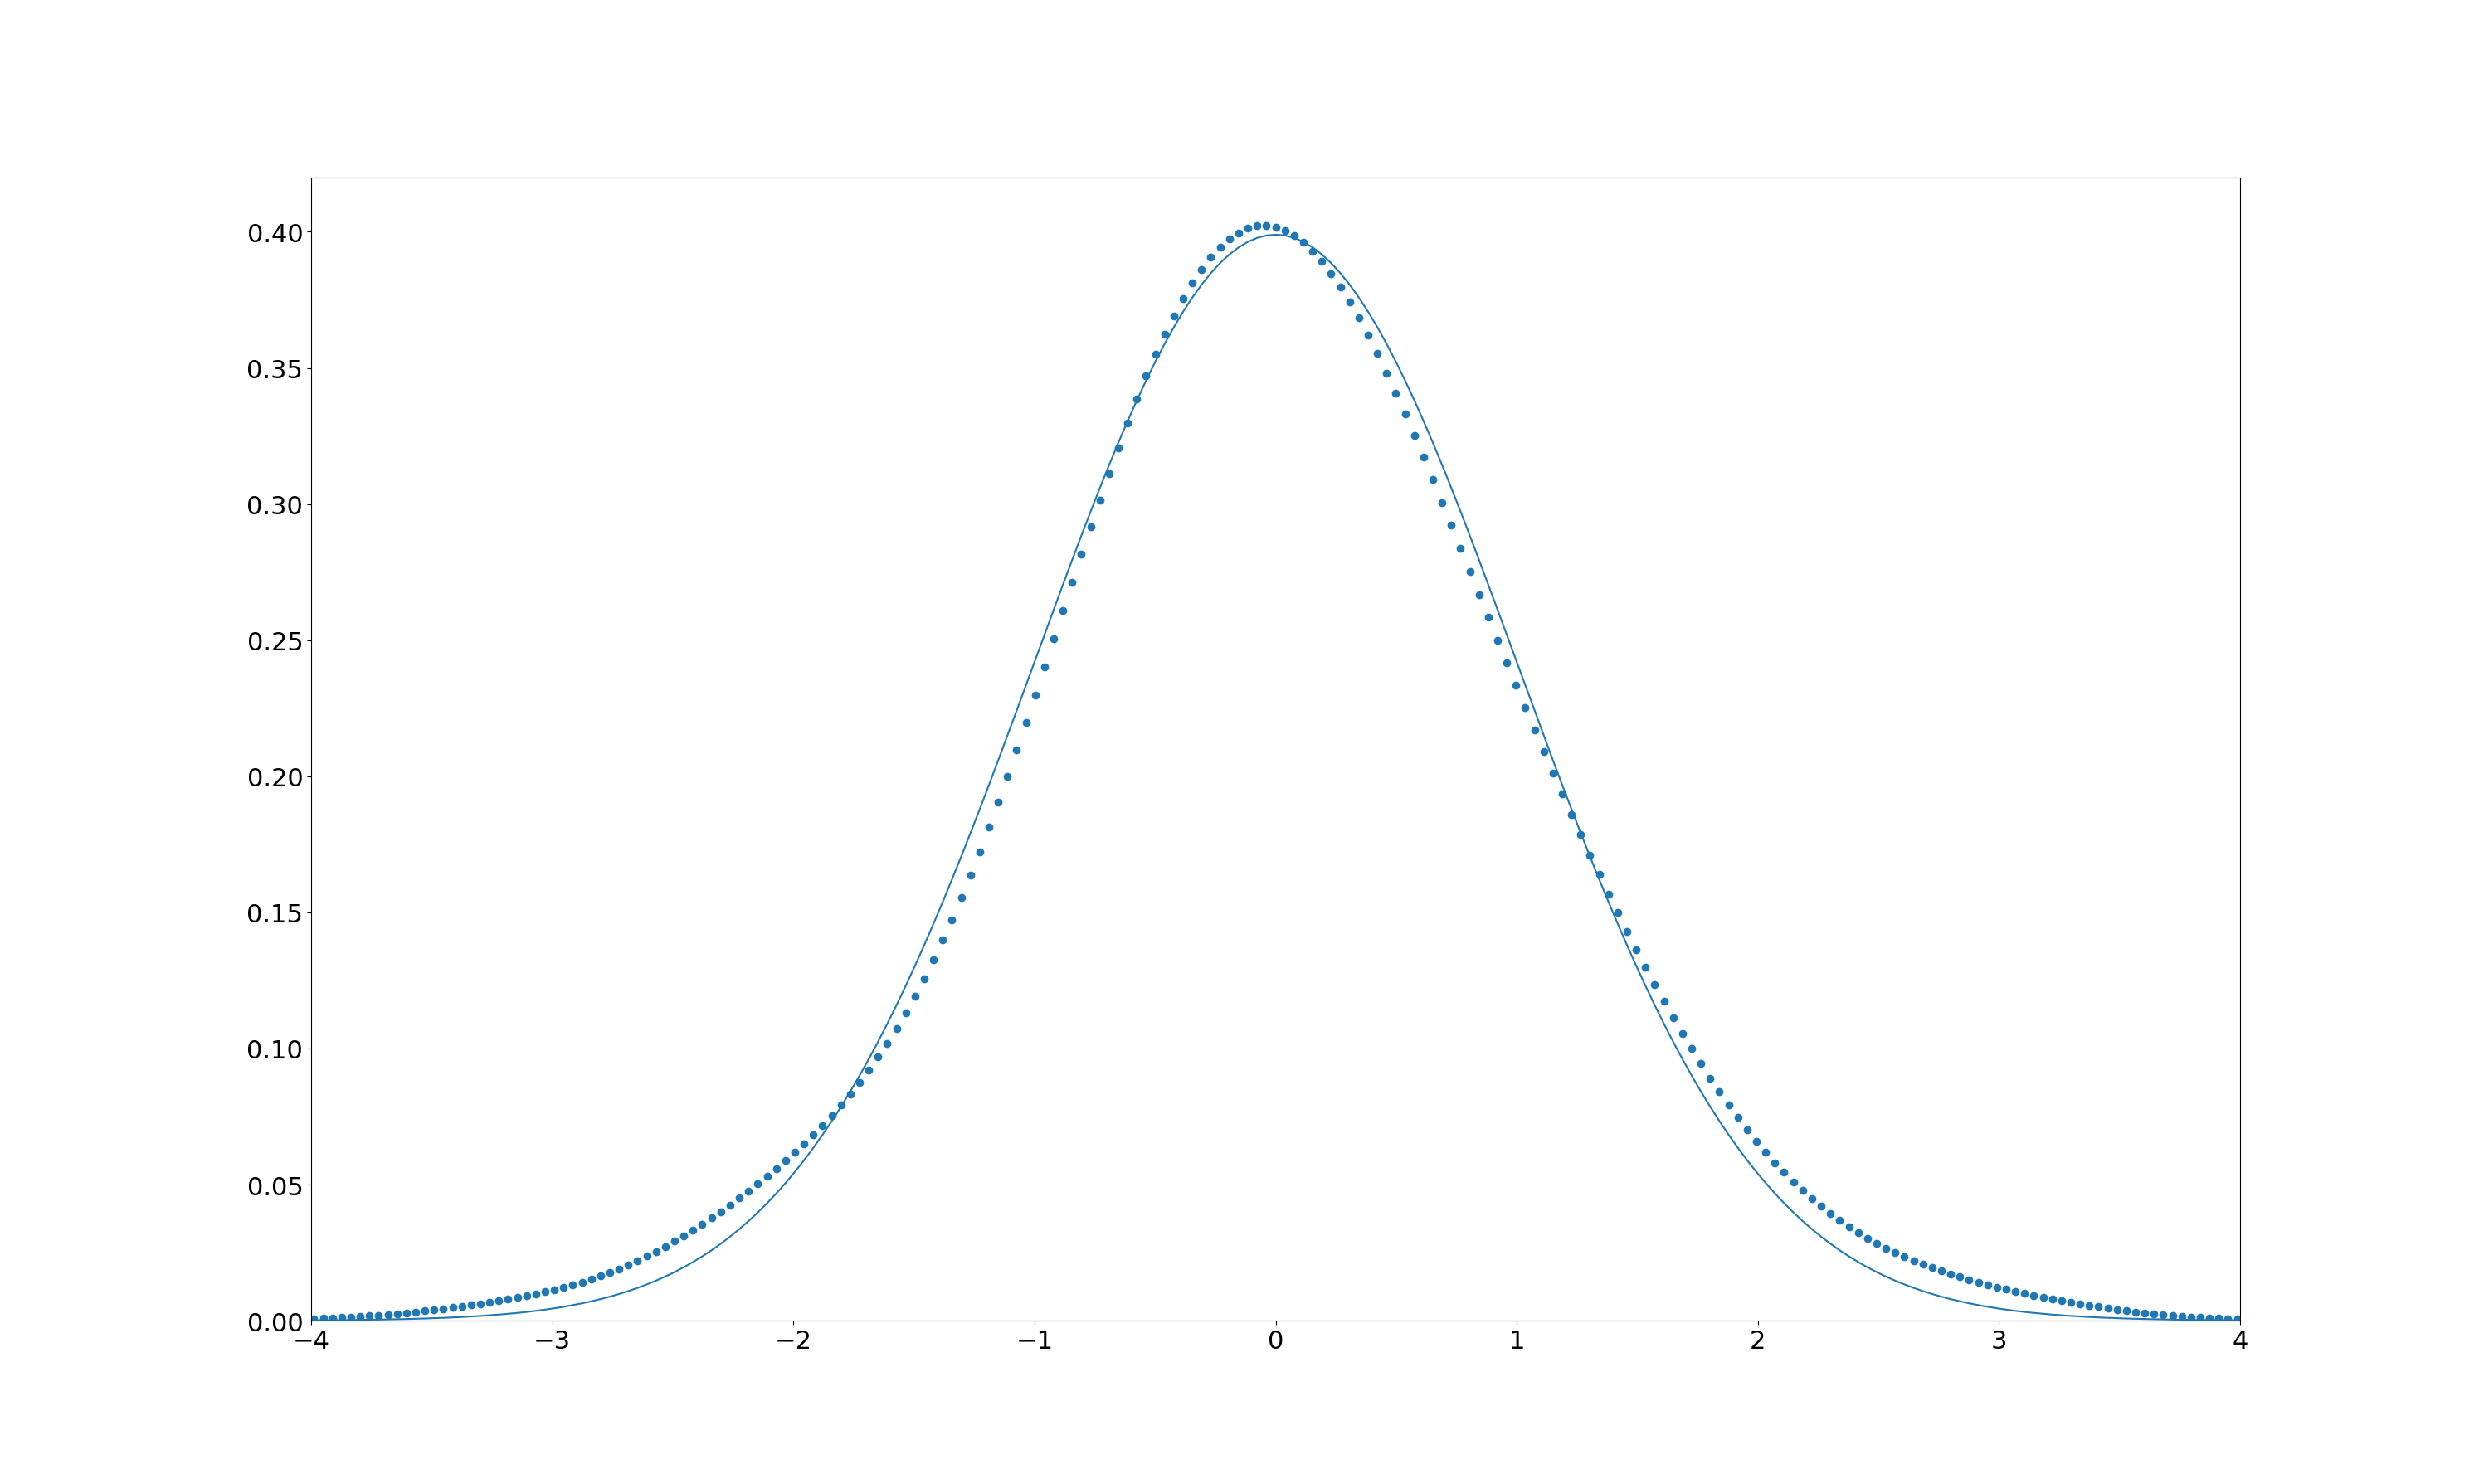
\includegraphics[scale=0.15]{spectralKDE.png}
\caption{Kernel Density Estimator for Standard Gaussian}
\label{stdNormal}
\end{figure} 

The second example we consider is the case of $f$ being a mixture of two normal densities
\[
f(\cdot) = \rho_{1}\psi(\cdot;\mu_{1},\sigma_{1}^{2}) + \rho_{2}\psi(\cdot;\mu_{2}, \sigma_{2}^{2}) 
\] 
where $\rho_{1} = \frac{3}{4}, \rho_{2} = \frac{1}{4}, \mu_{1} = 0, \mu_{2} = \frac{3}{2}, \sigma_{1}^{2} = 1, \sigma_{2}^{2} = \frac{1}{9}$. We use a bandwidth of 0.08 this time. The results are show in Figure \ref{MoG}.

\begin{figure}[h]
\centering
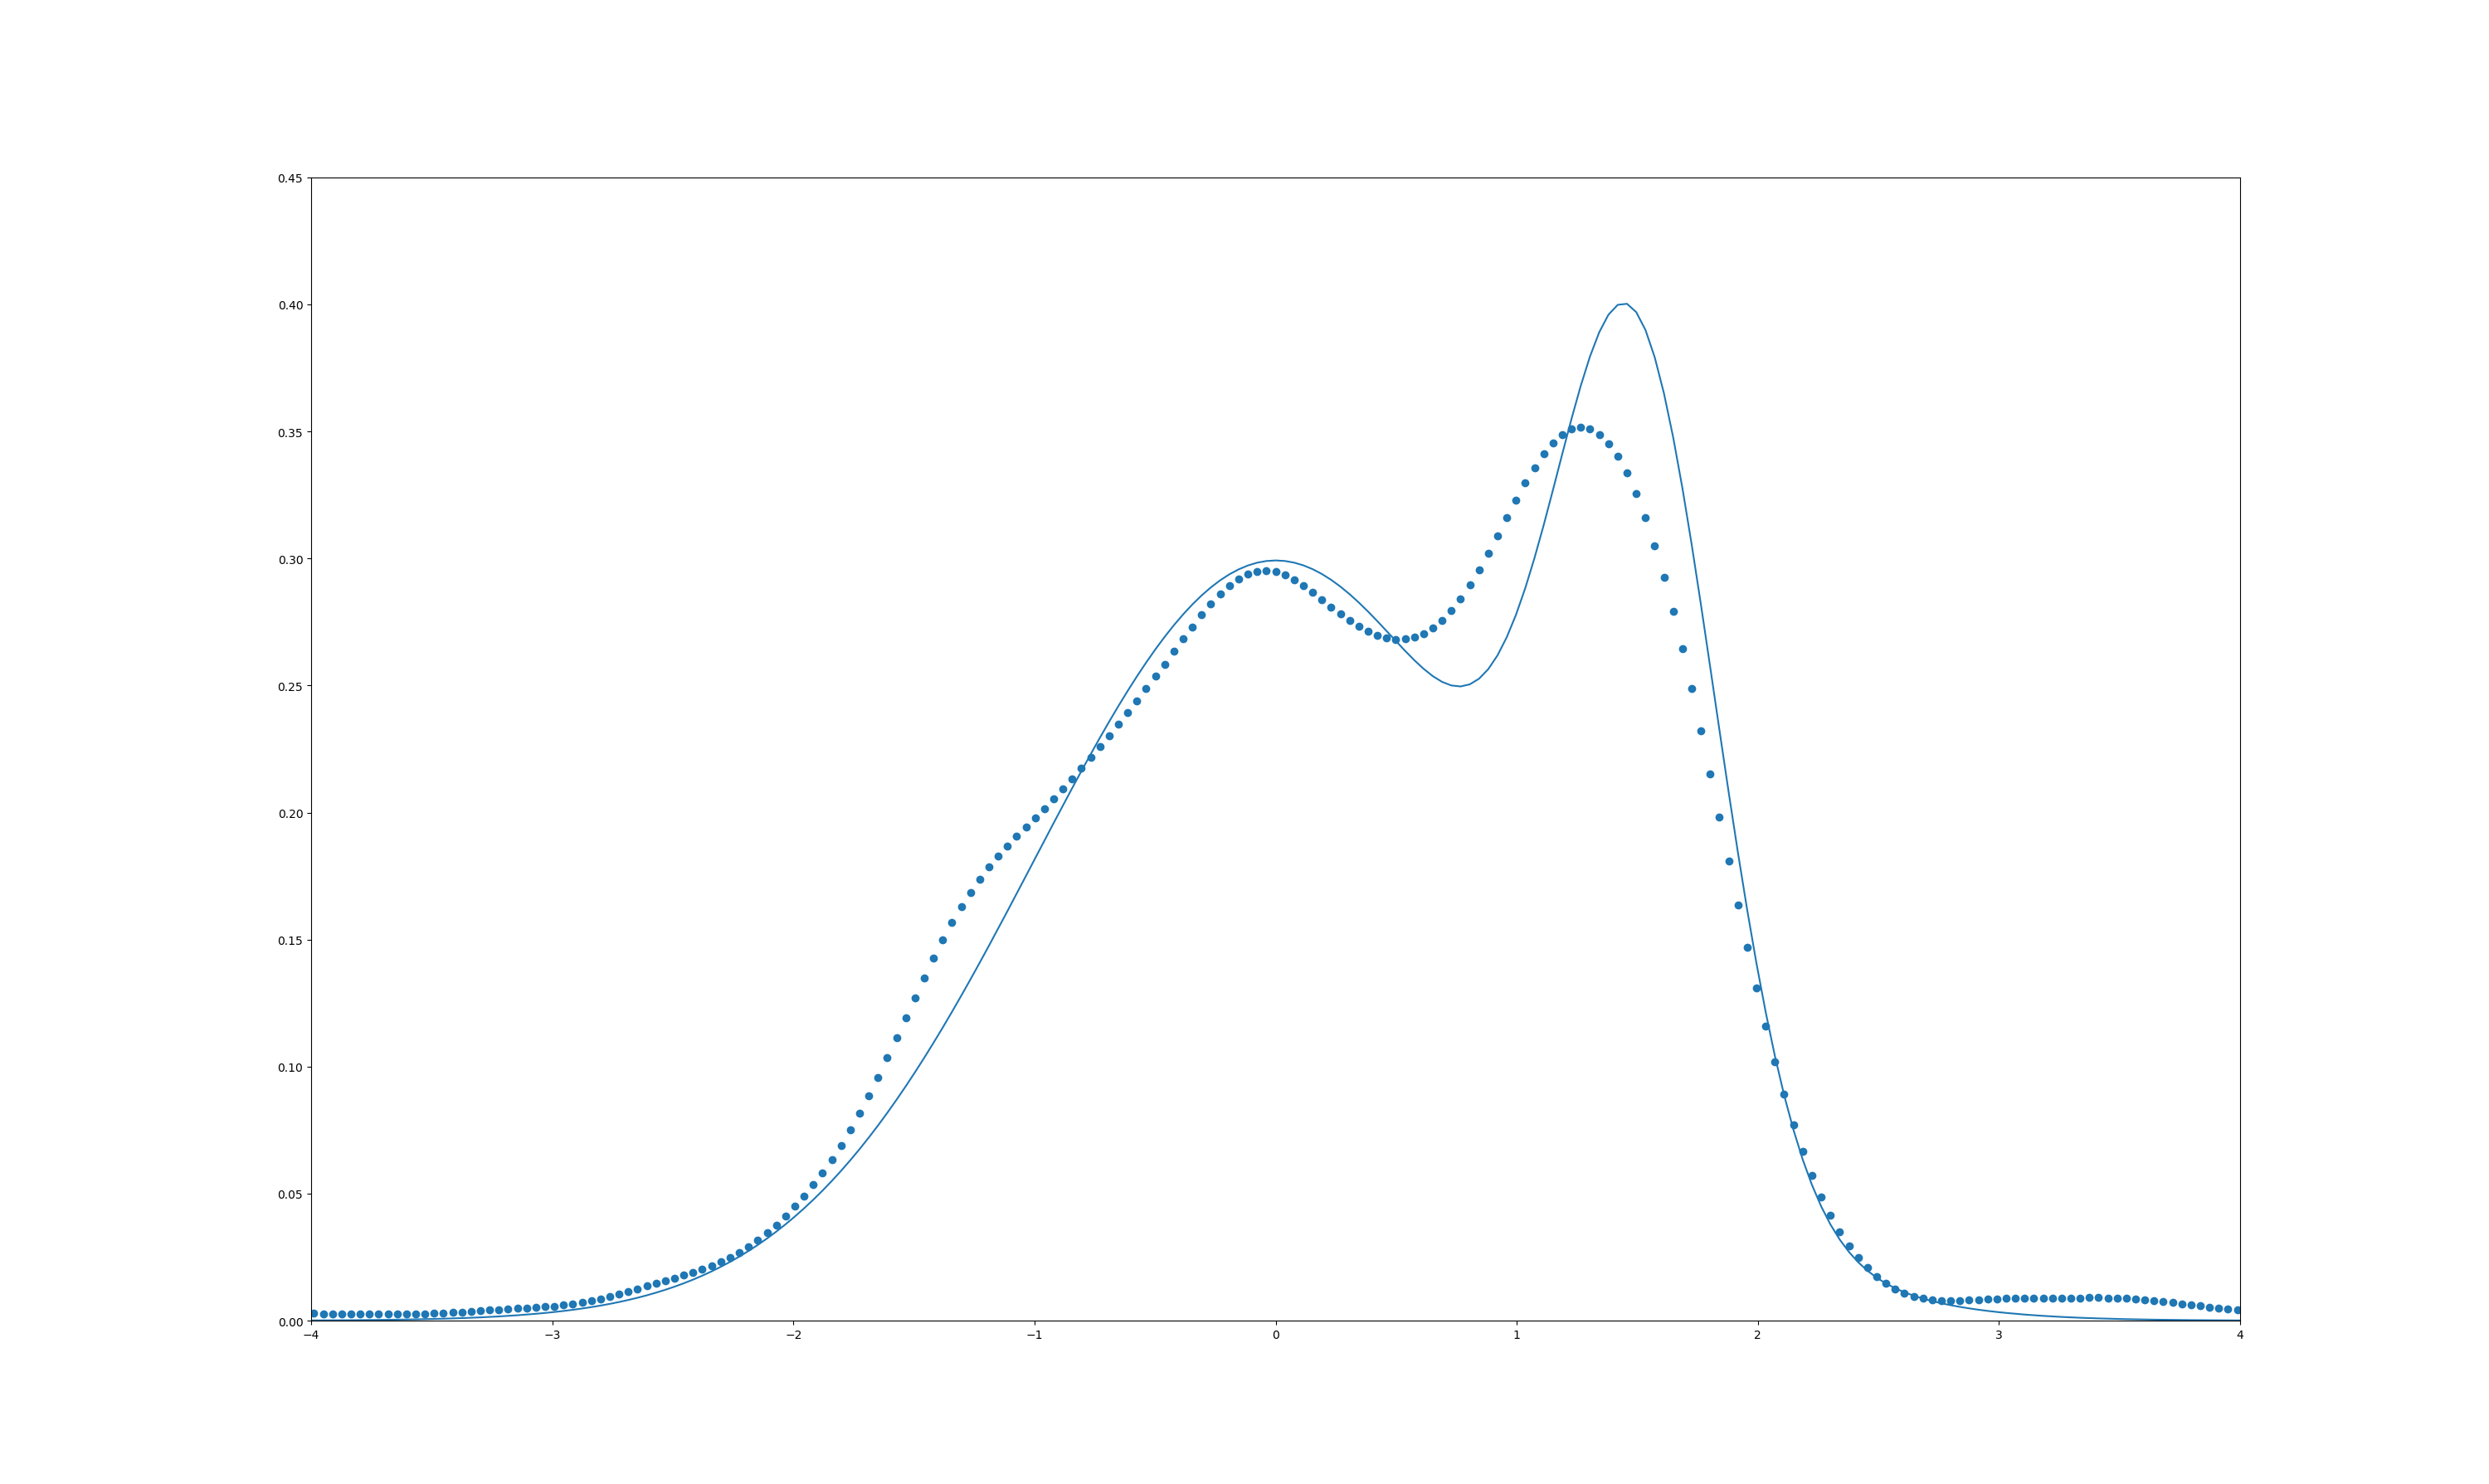
\includegraphics[scale=0.15]{spectralKDEMoG.png}
\caption{Kernel Density Estimator for Mixture of Gaussians}
\label{MoG}
\end{figure}

As shown, the estimator captures the bimodal nature of the dnesity $f$ in a fairly satisfactory manner.

\subsection{Comte}

We provide a different approach to tackling the problem of density estimation. Rather than looking at the characteristic function of the Poisson random sum $X$, we can, as shown by Duval, analytically provide an expression for the density of $X$ as being a sum of convolutions of the density $f$.

In particular, we see that given $N > 0$, the conditional density $g$ of $X | N > 0$ is given by

\begin{equation}
g(\cdot) = \sum_{m = 1}^{\infty}{a_m(\lambda \Delta) f^{\ast m}(\cdot)}
\end{equation}

We also see from (\ref{R-N duval}) that null increments provide no information on the density $f$. For fixed intensity $\lambda$ and $\Delta$, we see that the density $g$ depends only on $f$ so we can write $P(f) := g$. Therefore, if we can invert $P$ via some operator $P^{-1}$ to obtain $f = P^{-1}(g)$ then, given an estimator of $g$ we get a plug-in estimator for $f$. Amazingly, the operator $P$ can explicitly be inverted, provided $\lambda \Delta < \log 2$.

\begin{prop}
Provided that $\lambda \Delta < \log 2$, the inverse operator $P^{-1}$ of $P$ is well-defined and

\begin{equation}
f(\cdot) = P^{-1}(g)(\cdot) = \sum_{m=1}^{\infty}{\frac{(-1)^{m+1}}{m}\frac{(e^{\lambda \Delta} - 1)^m}{\lambda \Delta} g^{\ast m}(\cdot)}
\end{equation}
\end{prop}

\begin{proof}
Let $\mathcal{F}[f]$ denote the Fourier transform of $f$ and set $g := P[f]$. We note that $\mathcal{F} : L^{1}(\mathbb{R}) \to C_{0}(\mathbb{R})$ is injective. This is because, for $f \in L^{1}(\mathbb{R})$ such that $\mathcal{F}(f) = 0$, we have that $\mathcal{F}(f)$ is in $L^{1}(\mathbb{R})$ since it is the zero function. Therefore, its Fourier inverse exisits and so
\[
f = \mathcal{F}^{-1}(\mathcal{F}(f)) = \mathcal{F}^{-1}(0) = 0. 
\]
thus showing that $\mathcal{F}$ is injective on the space of Lebesgue-integrable functions, which is where our densities live.

The linearity of the Fourier transform and the relation $\mathcal{F}[f \ast g] = \mathcal{F}[f]\mathcal{F}[h]$ by the Convolution Theorem gives us that
\begin{align*}
\mathcal{F}[h] = \mathcal{F}\left[ P(f) \right] &= \frac{1}{e^{\lambda \Delta} - 1}\sum_{m=1}^{\infty}{\frac{(\lambda \Delta)^m}{m!} (\mathcal{F}[f])^m} \\
&= \frac{\exp\left(\lambda \Delta \mathcal{F}[f]\right) - 1}{e^{\lambda \Delta} - 1}
\end{align*}

Rearranging, we get that
\[
\exp\left(\lambda \Delta \mathcal{F}[f] \right) = 1 + (e^{\lambda \Delta} - 1) \mathcal{F}[h]
\]

Note that $\left\Vert (e^{\lambda \Delta} - 1)\mathcal{F}[h] \right\Vert_{\infty} < \left\Vert e^{\lambda \Delta} - 1 \right\Vert_{\infty} < 1$ for $\lambda \Delta < \log 2$. Therefore, the distinguished logarithm defined in the previous section reduces to the principal branch of the logarithm. Thus, we get that
\begin{equation} \label{inverse}
\mathcal{F}[f] = \frac{\log(1 + (e^{\lambda \Delta} - 1)\mathcal{F}[h])}{\lambda \Delta} = \sum_{m=1}^{\infty}{\frac{(-1)^{m+1}}{m}\frac{(e^{\lambda \Delta} - 1)^m}{\lambda \Delta} {\mathcal{F}[h]}^{m}}
\end{equation}
by the Taylor expansion of the logarithm, using the fact that $\lambda \Delta < \log 2$ implies that $\left\Vert (e^{\lambda \Delta} - 1)\mathcal{F}[h] \right\Vert_{\infty} < 1$.

Applying the inverse Fourier transform, since $f \in L^{1}(\mathbb{R})$, gives the result. 
\end{proof}

Note that for $\lambda \Delta < \log 2$, we have that the terms in the sum are pushed closer to 0 as $m$ gets larger. Therefore, it seems appropriate to consider a truncation of the series by keeping the first $K+1$ terms, where $K$ is sufficiently large, to give an approximation of $f$:
\begin{equation}
f(\cdot) \approx \sum_{m=1}^{K+1}{\frac{(-1)^{m+1}}{m}\frac{(e^{\lambda \Delta} - 1)^m}{\lambda \Delta} g^{\ast m}(\cdot)}
\end{equation}

In the paper of Chesneau, an estimator of the convolution power $g^{\ast m}$, given $n$ samples from the distribution that corresponds to density $g$.
We logically build the estimator and show its robustness on various simulations.

\subsubsection{Convolution Estimator}

Consider the kernel estimator for $g$ again:
\[
\hat{g}_{nh}(x) = \frac{1}{nh}\sum_{i=1}^{n}{K\left(\frac{x - Z_i}{h}\right)}
\] 

We take the kernel $K$ to be the sinus cardinal kernel, i.e.,
\[
K(x) = \frac{\sin(\pi x)}{\pi x}
\]

It is easy to compute that the characteristic function of this kernel is given by $\mathbbm{1}_{[-\pi, \pi]}(t)$. See Appendix.

Then a natural plug-in estimator for the characteristic function $\phi_{g}$ is $\phi_{\hat{g}_{nh}}$ and

\begin{equation}
\phi_{\hat{g}_{nh}}(t) = \int_{\infty}^{\infty}{\hat{g}_{nh}(x) e^{ixt} dx} = \phi_{\text{emp}}(t) \mathbbm{1}_{\left[-\frac{\pi}{h}, \frac{\pi}{h}\right]}(t)
\end{equation}
by (\ref{charformula}).

For i.i.d random variables $X_1, \dotsc, X_m$ with density $g$, we know that $X_1 + \dotsb + X_m$ has density $g^{\ast m}$ and $\phi_{g^{\ast m}}(t) = (\phi_{g}(t))^m$. Therefore, by Fourier inversion

\begin{equation}
g^{\ast m}(x) = \frac{1}{2\pi}\int_{\infty}^{\infty}{\phi_{g^{\ast m}}(t) e^{-itx} dt} = \frac{1}{2\pi}\int_{\infty}^{\infty}{(\phi_{g}(t))^m e^{-itx} dt}
\end{equation}

Therefore, our plug-in estimator for $g^{\ast m}$ is $\hat{g}_{nh}^{(m)}$ given by
\begin{align*}
\hat{g}_{nh}^{(m)}(x) &= \frac{1}{2\pi}\int_{\infty}^{\infty}{\left(\phi_{\text{emp}}(t) \mathbbm{1}_{\left[-\frac{\pi}{h}, \frac{\pi}{h}\right]}(t)\right)^{m} e^{-itx} dt} \\
&= \frac{1}{2\pi}\int_{-\frac{\pi}{h}}^{\frac{\pi}{h}}{\left(\phi_{\text{emp}}(t)\right)^{m} e^{-itx} dt}
\end{align*}

Therefore, we immediately get an estimator for $f$ given by
\begin{equation}
\hat{f}_{nh}(x) = \sum_{m=1}^{K+1}{\frac{(-1)^{m+1}}{m}\frac{(e^{\lambda \Delta} - 1)^m}{\lambda \Delta} \hat{g}_{nh}^{(m)}(x)}
\end{equation}

\subsubsection{Simulation Results}

As before, we approximate $\hat{g}_{nh}^{(m)}(x)$ by the trapezoid rule and then perform the FFT to compute $\hat{g}_{nh}^{(m)}(x)$ along a grid of values.

As we have done in the previous section, we rewrite $\hat{g}_{nh}^{(m)}(x) = \hat{g}_{nh}^{(m)(1)}(x) + \hat{g}_{nh}^{(m)(2)}(x)$ where
\begin{equation}
\hat{g}_{nh}^{(m)(1)}(x) = \frac{1}{2\pi}\int_{0}^{\frac{\pi}{h}}{\left(\phi_{\text{emp}}(t)\right)^{m} e^{-itx} dt}
\end{equation}

\begin{align*}
\hat{g}_{nh}^{(m)(2)}(x) &= \frac{1}{2\pi}\int_{-\frac{\pi}{h}}^{0}{\left(\phi_{\text{emp}}(t)\right)^{m} e^{-itx} dt} \\
&= \frac{1}{2\pi}\int_{0}^{\frac{\pi}{h}}{\left(\phi_{\text{emp}}(-t)\right)^{m} e^{itx} dt}
\end{align*}

We work with $\hat{g}_{nh}^{(m)(1)}$. The case for $\hat{g}_{nh}^{(m)(2)}$ is very similar. We approximate $\hat{g}_{nh}^{(m)(1)}(x)$ by taking a grid $t_j = j\eta$ for $j = 0,1,\dotsc, N-1$ where $N$ is some large power of 2 and $\eta = \frac{\pi}{(N-1)h}$.
\begin{equation}
\hat{g}_{nh}^{(m)(1)}(x) \approx \frac{1}{2\pi}\sum_{j=0}^{N-1}{\left(\phi_{\text{emp}}(t_j)\right)^m e^{-it_j x} \eta}
\end{equation}

We take $x_k = -\frac{N\delta}{2} + \delta k$ for $k = 0, 1, \dotsc, N-1$ and $\delta$ is some constant to be defined later. Then
\[
\hat{g}_{nh}^{(m)(1)}(x) \approx \frac{1}{2\pi}\sum_{j=0}^{N-1}{\left(\phi_{\text{emp}}(t_j)\right)^m e^{it_j \frac{N\delta}{2}} e^{-ijk\eta\delta} \eta}
\]

Similarly,
\[
\hat{g}_{nh}^{(m)(2)}(x) \approx \frac{1}{2\pi}\sum_{j=0}^{N-1}{\left(\phi_{\text{emp}}(-t_j)\right)^m e^{-it_j \frac{N\delta}{2}} e^{ijk\eta\delta} \eta}
\]

We choose $\delta = \frac{2h(N-1)}{N}$ so that $\eta\delta = \frac{2\pi}{N}$ and then apply FFT (or IFFT) to these terms to obtain an estimate for $\hat{g}_{nh}^{(m)}$.

\section{Bayesian Approach}

We now consider the non-parametric Bayesian approach to estimating 'true' parameter values $f_{0}$ as well as $\lambda_{0}$ from discrete evenly-spaced observations of the CPP.

The advantages of using a non-parametric Bayesian approach are two-fold:
\begin{enumerate}
\item We obtain a distribution over all probability densities rather than just a point estimate as in the spectral approach,
\item We obtain automatic uncertainty quantification through the posterior credible sets
\end{enumerate}

\subsection{Bayesian Nonparametrics}

In the Bayesian framework, the data $X$ follows a distribution determined by a parameter $\theta$, which is itself considered to be generated from a prior distribution $\Pi$. The corresponding posterior distribution is the conditional distribution of $\theta$, given $X$. This framework is identical in parametric and nonparametric Bayesian statistics, the only difference being the dimension of the parameter $\theta$.

Because, in the nonparametric case, the prior distribution is a distribution over an infinite-dimensional space, we must carefully construct the setup in order to apply Bayes Theorem.

Let $(\mathcal{F}, \mathcal{B})$ be a measurable space, where $\mathcal{F}$, in our following discussion, will be a set of functions denoting the parameter space. Then the prior distribution $\Pi$ is a probability measure on $(\mathcal{F}, \mathcal{B})$.

Let $(\mathfrak{X}, \mathcal{X})$ denote our sample space. Suppose we have data $X$ - this data is a random variable from some probability space $(\Omega, \mathcal{A}, \mathbb{P})$ so $X: \Omega \to \mathfrak{X}$. Our model/likelihood $P_{\theta}$ of $X$ given $\theta$ is a Markov kernel with source $(\mathcal{F}, \mathcal{B})$ and target $(\mathfrak{X}, \mathcal{X})$. 

\begin{defn}
Let $(X, \mathcal{A}), (Y, \mathcal{B})$ be measurable spaces. A Markov kernel with source $(X, \mathcal{A})$ and target $(Y, \mathcal{B})$ is a map $\kappa : X \times \mathcal{B} \to [0, 1]$ with the following properties:
\begin{enumerate}
\item The map $x \mapsto \kappa(x, B)$ is $(X, \mathcal{A})$-measurable for every $B \in \mathcal{B}$
\item The map $B \mapsto \kappa(x, B)$ is a probability measure on $(Y, \mathcal{B})$ for every $x \in X$.
\end{enumerate} 
\end{defn}

Therefore, $A \mapsto P_{\theta}(A)$ is a probability measure on $(\mathfrak{X}, \mathcal{X})$.

For pair $(X, \theta)$, we have a well-defined joint distribution on the product space $(\mathcal{F} \times \mathfrak{X}, \mathcal{B} \otimes \mathcal{X})$ given by
\[
P(B, A) = P(\theta \in B, X \in A) = \int_{B}{P_{\theta}(A)d\Pi(\theta)}
\]   
and we note that the integral is well-defined since the map $\theta \mapsto P_{\theta}(A)$ is $(\mathcal{F}, \mathcal{B})$-measurable.

From this we get the marginal distribution of $X$ given by
\[
P(X \in A) = \int{P_{\theta}(A)d\Pi(\theta)}
\]
i.e. a probability measure $P_{X}$ on $(\mathfrak{X}, \mathcal{X})$
\[
P(\theta \in B | X) = \E_{P} \left[ \mathbbm{1}(\theta \in B) \;|\; \sigma(X) \right] \qquad \text{a.s.}
\]

Note that $\sigma(X) = \mathcal{X}$ and we can write the posterior distribution $\Pi(B|X) = P(\theta \in B | X)$. Under certain conditions, there exists a regular version of the conditional distribution i.e. a Markov kernel $\mu$ from source $(\mathfrak{X}, \mathcal{X})$ and target $(\mathcal{F}, \mathcal{B})$ such that the map $B \mapsto \mu(x, B)$ is a probability measure on $(\mathcal{F}, \mathcal{B})$ and equals $\Pi(B|X)$ almost surely.   

A sufficient condition for this is when $\mathcal{F}$ is a Polish space equipped with Borel $\sigma$-algebra $\mathcal{B}$.


 
\subsection{Gugushvili}

We consider the problem of estimating density $f_{0}$ from the non-parametric class $\mathcal{F}$ of location-scale mixtures of normal densities.

\subsubsection{Mixtures} \label{mixtures}

A powerful technique, especially for computation, is to construct a prior on probability densities is through mixtures.

For given probability density functions $\{ \psi_{\theta} : \theta \in \Theta\}$ (such that the map $x \mapsto \psi_{\theta}(x) = \psi(\theta, x)$ is measurable in both arguments) and a probability distribution $F$ on the parameter space $(\Theta, \mathcal{T})$, let
\[
p_{F}(x) = \int{f(\theta, x) dF(x)}
\]

Then a prior on $F$ induces a prior on densities. The function $\psi$ is referred to as the kernel function and the measure $F$ is called the mixing distribution. 

In our case we use a location-scale mixture of normal densities. Therefore, our kernel is of the form $x \mapsto \frac{1}{\sigma}\psi\left(\frac{x- \mu}{\sigma}\right)$ where $\psi$ denotes the probability density function of a standard normal and $\theta = (\mu, \sigma)$.

Such a family is rich since by Fejer's theorem,

\[
\int{\frac{1}{\sigma}\psi\left(\frac{x- \mu}{\sigma}\right) f(\mu)d\mu} \to f(\cdot) \text{ as } \sigma \to 0 \text{ in } L^1
\]

Thus, a prior on densities may be induced by putting a prior on the mixing distribution $F$ and a prior on $\sigma$ restricted to positive values.

The mixing distribution $F$ may be given a Dirichlet process prior since it leads to efficient computational algorithms as well as rich convergence properties. Thus, for our discussion, such a prior is particularly attractive. 

\subsubsection{Priors on Spaces of Probability Measures}

As we have seen in the previous section, placing a prior on the mixing distribution $F$ induces a prior on the space of probability densities. This construction comes with some technical complications.

We provide a rigorous discussion of its construction nad then introduce methods of constructing priors, in particular stick breaking and the P\'{o}lya urn scheme.

Let $(\mathfrak{X}, \mathcal{X})$ be a Polish space and consider priors on the collection $\mathfrak{M}$ of all probability measures on $(\mathfrak{X}, \mathcal{X})$. A prior $\Pi$ on $\mathfrak{M}$ can be viewed as the distribution of a \textit{random measure} $P$.

\begin{defn}
A random measure, in this case, can be thought of as a random element from some probability space $(\Omega, \mathcal{F}, \mathbb{P})$ to our collection of probability measures $(\mathfrak{M}, \mathcal{B}(\mathfrak{M}))$ equipped with a suitable Borel $\sigma$-field. This is equivalent to being a (a.s.) locally finite Markov kernel from a probability space $(\Omega, \mathcal{F}, \mathbb{P})$ to our sample space $(\mathfrak{X}, \mathcal{X})$. 
\end{defn} 

Thus we can view $P$ as a map $P: \Omega \times \mathcal{X} \to \mathbb{R}$ such that $P_{\omega}$ is a measure on $(\mathfrak{X}, \mathcal{X})$ for every $\omega \in \Omega$. Thus $P_{\omega} \in \mathfrak{M}$.

Now, also from the definition, for fixed $A \in \mathcal{X}$, $P(A) : \Omega \to \mathbb{R}$ is a random variable. Therefore, we get that $(P(A) : A \in m\mathcal{X})$ is a stochastic process on the underlying probability space $(\Omega, \mathcal{F}, \mathbb{P})$.

Then $\Pi$ is a measure on $(\mathfrak{M}, \mathcal{M})$ where $\mathcal{M}$ is some Borel $\sigma$-field for the weak topology etc... and it makes sense to talk about

\[
\Pi(M) = \text{Pr}(P \in M) 
\]

for some probability measure Pr on $(\mathfrak{M}, \mathcal{M})$. Therefore, we can speak of drawing a measure $P$ from the prior $\Pi$ and then sampling observations $X \in \mathfrak{X}$ from $P$.

\subsubsection{Countable Sample Spaces}

A probability distribution on a countable sample space (equipped with the $\sigma$-field of all its subset) can be represented as a infinite-length probability vector $s = (s_1, s_2, \dotsc)$ , thus assigning probability weights to each element in the sample space. This can be trivially seen in, for example, a Poisson distribution where we get the probability vector:
\[
\left(e^{-\lambda}\frac{\lambda^{k}}{k!}\right)_{k=0}^{\infty}
\]

Therefore, a prior on the set $\mathfrak{M}$ of all probability measures on a countable sample space can therefore be identified with the distribution of a random element with values in the countable-dimensional unit simplex
\begin{equation}
\mathbb{S}_{\infty} = \left\lbrace s = (s_1, s_2, \dotsc): s_j \geq 0, j \in \mathbb{N}, \sum_{j=1}^{\infty}{s_j} = 1\right\rbrace
\end{equation}

Characterising the $\sigma$-field on $\mathbb{S}_{\infty}$ by the $\sigma$-algebra generated by the coordinate maps $s \mapsto s_{i}, i \in \mathbb{N}$, then this shows that a map $p$ from some probability space into $\mathbb{S}_{\infty}$ is a random element if and only if every coordinate variable $p_{i}$ is a random variable. Hence a prior corresponds to an infinite sequence of nonnegative random variables $p_1, p_2, \dotsc$ that add up to 1.

We can use this fact to sample from our prior $\Pi$ by obtaining a sequence $Y_1. Y_2, \dotsc$ of random variables such that their sum $\sum_{i=1}^{\infty}{Y_{i}} = 1$. We do this via several methods.

\subsubsection{Construction through Normalization}

Given nonnegative random variables $Y_1, Y_2, \dotsc$ such that $\sum_{j=1}^{\infty}{Y_j}$ is positive and converges a.s. we can define a prior on $\mathbb{S}_{\infty}$ by putting
\begin{equation} \label{normalization}
p_k = \frac{Y_k}{\sum_{j=1}^{\infty}{Y_j}}, \qquad k \in \mathbb{N}
\end{equation}

A simple sufficient condition for the a.s. convergence of the random series is that $\sum_{j=1}^{\infty}{\E (Y_j)} < \infty$. The construction follows by the following lemma:

\begin{lem}
If $Y_1, Y_2, \dotsc$ are independent, positive random variables with $\sum_{j=1}^{\infty}{Y_j} < \infty$ a.s. and marginal densities, i.e. the density of $(Y_i)_{i \in I}$ where $I \subset \mathbb{N}$, is positive everywhere in $(0, \infty)$, then the support of the prior defined by (\ref{normalization}) is equal to the full space $\mathbb{S}_\infty$. 
\end{lem}  

\subsubsection{Construction through Stick Breaking}

We perform the following algorithm to distribute the total mass 1, conceptually visualised with a stick of length 1, randomly to each element of $\mathbb{N}$.
\begin{enumerate}
\item We first break the stick at the point given by the random variable $V_1$ where $0 \leq V_1 \leq 1$ and assign mass $V_1$ to $p_1$.
\item We think of the remaining mass $1 - V_1$ as a new stick and break it into two pieces of relative lengths $V_2$ and $1 - V_2$ according to the value of random variable $V_2$. We assign mass $(1 - V_1)V_2$ to the point $p_2$
\item We repeat in this way so that point $p_j$ has mass
\begin{equation} \label{stickbreak}
p_j = \left(\prod_{l=1}^{j-1}{(1-V_l)}\right)V_j
\end{equation}

\end{enumerate}

\subsubsection{Countable Dirichlet Process}

We construct the countable Dirichlet distribution via stick breaking:
WE choose the variables $V_1, V_2, \dotsc$ independently with $V_j \sim \text{Be}(\alpha_j, \sum_{l=j+1}^{\infty}{\alpha_l}$ and define $(p_1, p_2, \dotsc )$ by (\ref{stickbreak}).

It follows easily that for any $k \in \mathbb{N}$,

\begin{equation}
\left(p_1, \dotsc, p_k, 1 - \sum_{j=1}^{k}{p_j}\right) \sim \text{Dir}\left(k+1; \alpha_1, \dotsc, \alpha_k, \sum_{j=k+1}^{\infty}{\alpha_j}\right)
\end{equation}
and so we have a Dirichlet Process

\begin{defn}
A random measure $P$ on $(\mathfrak{X}, \mathcal{X})$ is said to possess a Dirichlet process distribution DP($\alpha$) with base measure $\alpha$ on the measurable space $(\mathfrak{X}, \mathcal{X})$ if, for every finite measurable partition $A_1, \dotsc, A_k$ of $\mathfrak{X}$, we have that the joint distribution of random variables $P(A_1), \dotsc, P(A_k)$ satisfy
\[
(P(A_1), \dotsc, P(A_k)) \sim \text{Dir}\left(k+1; \alpha(A_1), \dotsc, \alpha(A_k)\right) 
\]
\end{defn}

Therefore, in our case, the random variables $(p_1, p_2, \dotsc )$ follow a Dirichlet process.

Suppose that we have a sample of i.i.d observations $X_1, \dotsc, X_n$ from $p$.
The likelihood $L$, therefore, is given by
\[
L(p) = \prod_{j=1}^{\infty}{p_{j}^{N_j}}
\]
where $N_j = \sum_{i=1}^{n}{X_{i}^{(j)}}$ i.e the sum of the $j$th component of all the observations.

The vector $N = (N_1, N_2, \dotsc)$ is a sufficient statistic, and hence the posterior given $N$ is the same as the posterior given the original observations.

For any $l \in \mathbb{N}$,
\begin{equation} \label{multiNom}
\left( N_1, N_l, n - \sum_{j=1}^{l}{N_j}\right) \sim \text{MN}_{l+1}\left(n; p_1, \dotsc, p_l, 1 - \sum_{j=1}^{\infty}{p_j}\right).
\end{equation}

By conjugacy of the finite Dirichlet distribution with the multinomial likelihood, we get that the posterior density of $(p_1, \dotsc, p_l, 1- \sum_{j=1}^{l}{p_j})$ given $N_1, \dotsc, N_l$ is given by
\[
\text{Dir}\left(l+1; \alpha_1 + N_1, \dotsc, \alpha_l + N_l, \sum_{j=l+1}^{\infty}{\alpha_j} + n - \sum_{j=1}^{l}{N_j}\right)
\]

Using part (i) of Proposition G.3, we can aggregate entries in the last cell on a partition $\{1\}, \dotsc, \{k\}, \{k+1, k+2, \dotsc \}$ for $(k \leq l)$ to give that the posterior density of $\left(p_1, \dotsc, p_k, 1 - \sum_{j=1}^{k}{p_j}\right)$ given $N_1, \dotsc, N_l$ is given by
\[
\text{Dir}\left(k+1; \alpha_1 + N_1, \dotsc, \alpha_k + N_k, \sum_{j=k+1}^{\infty}{\alpha_j} + n - \sum_{j=1}^{k}{N_j}\right)
\]

Since this density only depends on $N_1, dotsc, N_k$ we get that this posterior density of $\left(p_1, \dotsc, p_k, 1 - \sum_{j=1}^{k}{p_j}\right)$ given $N_1, \dotsc, N_l$ is the same for every $l \geq k$. Thus, since we have that $\sigma(N_1, \dotsc, N_l)$ is a filtration in $l$ and $\sigma(N)$ is the minimal $\sigma$-algebra generate by this filtration then by L\'{e}vy's zero-one law, the above posterior density is the same for $\left(p_1, \dotsc, p_k, 1 - \sum_{j=1}^{k}{p_j}\right)$ given $N$.

The posterior parameters depend on the prior parameters and the new parameter is given simply by $\alpha \mapsto \alpha + N$ (element-wise).

In analogy with thte finite dimensional Dirichlet distribution, it is natural to call the prior the \textit{Dirichlet process} on $\mathbb{N}$ (or the \textit{countable Dirichlet process}. We shall write $(p_1, p_2, \dotsc) \sim \text{DP}(\alpha)$ where $\alpha = (\alpha_1, \alpha_2, \dotsc )$.

From the properties of the finite-dimensional Dirichlet distribution, the posterior mean can be written as
\[
\E \left(p_j | X_1, \dotsc, X_n \right) = \frac{a_j + N_j}{\sum_{l=1}^{\infty}{a_l} + n}
\]
This seems intuitively correct, since higher $N_j$ will provide a greater mass on $p_j$.

\subsubsection{Dirichlet Process on Arbitrary Sample Spaces}

We saw previously that for a countable Dirichlet process prior, the posterior distribution is again a countable Dirichlet process. This result extends also to Dirichlet process on an arbitrary space.

Consider observations $X_1, X_2, \dotsc, X_n$ sampled independently from a distribution $P$ that was drawn from a Dirichlet prior distribution. By some abuse of language, we will say that this sample is from the Dirichlet process.

\begin{thm}
(Conjugacy) The DP$\left(\alpha + \sum_{i=1}^{n}{\delta_{X_i}}\right)$ process is a version of the posterior distribution given an i.i.d sample $X_1, \dotsc, X_n$ from the DP($\alpha)$-process.
\end{thm}

\subsubsection{Construction through P\'{o}lya Urn Scheme}

\begin{enumerate}
\item $X_1 \sim \bar{\alpha}$
\item $X_{n+1} | X_1, \dotsc, X_n \sim \frac{\alpha + \sum_{i=1}^{n}{\delta_{X_i}}}{|\alpha| + n}$
\end{enumerate}

By de Finetti's theorem, there exists a random probability measure $P$ such that $X_i | P \overset{\text{i.i.d}}{\sim} P$. We see in Section 4.2.4 that the law of $P$ is the DP($\alpha$)-process.

\subsubsection{Stick-Breaking Representation}

The stick-breaking representation of a Dirichlet process expresses it as a random discrete measure with stick-breaking weights, based on the beta-distribution.

The representation gives an easy method to simulate a Dirichlet process, at least approximately. We use this to simulate our Dirichlet process

\begin{thm}
If $\theta_1, \theta_2, \dotsc \overset{\text{iid}}{\sim}\bar{\alpha}$ and $V_1, V_2, \dotsc \overset{\text{i.i.d}}{\sim} \text{Be}(1, M)$ are independent random variables and $W_j = V_j\prod_{l=1}^{j-1}{(1-V_l)}$ then $\sum_{j=1}^{\infty}{W_j\delta_{\theta_j}} \sim \text{DP}(M\bar{\alpha})$.
\end{thm}

Note that
\begin{thm}
(Discreteness) Almost every realization from the DP($\alpha$) is a discrete measure: $\text{DP}_{\alpha}(P \in \mathfrak{M}: P \text{ is discrete}) = 1$.
\end{thm}

This is perhaps disappointing, especially if the intention is to model absolutely continuous probability measures. In particular, the Dirichlet process cannot be used as a prior for density estimation. We therefore actually use a Dirichlet Process mixture.

\subsubsection{Dirichlet Process Mixtures}

The discreteness of the Dirichlet process makes it useless as a prior for estimating a density. This can be remedied by convolving it with a kernel. Although it is rarely possible to characterize the resulting posterior distribution analytically, a variety of efficient and elegant algorithms allows us to approximate it numerically.

We follow the same definition in Section \ref{mixtures} with $F$ equipped with Dirichlet process prior but we also allow the kernel to depend on an additional parameter $\phi \in \Phi$, giving mixtures $p_{F, \phi}(x) = \int{\psi_{i}(x;\theta, \phi)dF(\theta)}$.

For $x \mapsto \psi_i(x;\theta,\phi)$ probability density functions (relative to a given $\sigma$-finite dominating measure $\nu$, consider

\[
X_i \overset{\text{i.i.d}}{\sim} p_{i, F, \phi}(x) = \int{\psi_i(x; \theta, \phi)dF(\theta)} 
\]

We equip $F$ and $\phi$ with independent priors $F \sim \text{DP}(\alpha)$ and $\phi \sim \pi$.

The resulting model can be equivalently written in terms of $n$ latent variables $\theta_1, \dotsc, \theta_n$ as

\begin{equation} \label{model}
X_i | \theta_i, \phi, F \overset{\text{ind}}{\sim} \psi_i(\cdot; \theta_i, \phi), \qquad \theta_i | F, \phi \overset{\text{iid}}{\sim} F, \qquad F \sim \text{DP}(\alpha), \qquad \phi \sim \pi
\end{equation}

The latent variables $\theta_1, \dotsc, \theta_n$ help to make the description simpler, since $F | \theta_1, \dotsc, \theta_n \sim \text{DP}(\alpha + \sum_{i=1}^{n}{\delta_{\theta_i}})$

The posterior distribution of any object of interest can be described in terms of the posterior distribution of $(F, \phi)$ given $X_1, \dotsc, X_n$.

Note that for any measurable function $\psi$
\begin{equation} \label{condExp}
\E \left[ \int{\psi dF | \theta_1, \dotsc, \theta_n, X_1, \dotsc, X_n} \right] = \frac{1}{|\alpha| + n}\left[\int{\psi d\alpha} + \sum_{j=1}^{n}{\psi(\theta_j)}\right]
\end{equation}

We use this to simulate from the posterior distribution of $(\theta_1, \dotsc, \theta_n)$ based on a weighted generalized P\'{o}lya urn scheme.

\begin{thm}
(Gibbs sampler) In the model (\ref{model}) the conditional posterior distribution of $\theta_i$ is given by
\begin{equation}
\theta_i | \theta_{-1}, \psi, X_1, \dotsc, X_n \sim \sum_{j \neq i}{q_{i,j} \delta_{\theta_j} + q_{i,0}G_{b,i}} 
\end{equation}
where $(q_{i,j}:j \in \{0,1, \dotsc, n\} \setminus \{i\})$ is the probability vector satisfying
\[
q_{i,j} \propto 
\begin{cases}
\psi_{i}(X_i;\theta_j, \phi), & j \neq i, j \geq 1, \\
\int{\psi_{i}(X_i; \theta, \phi)d\alpha(\theta)}, & j = 0,
\end{cases}
\]
and $G_{b,i}$ is the baseline posterior measure given by
\[
dG_{b,i}(\theta | \phi, X_i) \propto \ \psi_{i}(X_i; \theta, \phi)d\alpha(\theta)
\]
\end{thm}

See MCMC Methods in section 5.2 to simulate from the posterior distribution in the Dirichlet process. The basic algorithm uses the Gibbs sampling in above theorem to generate $\theta_1, \dotsc, \theta_n$ given $X_1, \dotsc, X_n$ and then we can readily obtain the posterior $F$ given $X_1, \dotsc, X_n$.

\subsection{Gugushvili Problem Formulation}

We consider the problem of estimating density $f_{0}$ from the non-parametric class $\mathcal{F}$ of location mixtures of normal densities. These are not location-scale since we fix $\sigma$.

\begin{eg}
Consider distribution $F$ on $(\mathbb{R}, \mathcal{B})$ given by
\[
F(\cdot) = \sum_{j=1}^{n}{p_j\delta_{\mu_j}(\cdot)}
\]  
where $\sum_{j=1}^{n}{p_j} = 1$ and $\delta_{\mu_i}$ denotes the dirac measure centred at $\mu_i \in \mathbb{R}$.

Then we get that
\[
\int{\frac{1}{\sigma}\psi\left(\frac{x- \mu}{\sigma}\right)dF(\mu)} = \sum_{j=1}^{n}{p_j\frac{1}{\sigma}\psi\left(\frac{x- \mu_j}{\sigma}\right)}
\]
so we get a weighted sum of normal densities. Therefore, mixtures basically generalise this idea of returning a weighted sum of densities from a specific parametric family.
\end{eg}

\subsubsection{Prelims and Notation}

Let $\mathbb{P}_{f}$ be the law of the jumps $Y_1$ of the CPP.

Let $\mathbb{Q}_{\lambda, f}^{\Delta}$ be the law of the increments $Z_1$ of the discretely observed points of the CPP. These $Z_i$ have same distribution as a Poisson random sum

Let $\mathbb{Q}_{\lambda, f}^{\Delta, n}$ be the joint law of the increments $\mathcal{Z}_{n}^{\Delta} = (Z_{1}^{\Delta}, \dotsc, Z_{n}^{\Delta})$ of the discretely observed points of the CPP.

Let $\mathbb{R}_{\lambda, f}^{\Delta}$ be the law of $(X_t : t \in [0, \Delta])$ i.e. the law of the CPP restricted to interval $[0, \Delta]$.

By (\ref{characteristicPS}) (we need to change it to consider $\Delta$) we know that the characteristic function of the Poisson random sum $X$ is given by
\[
\phi_{X}(t) = e^{-\lambda \Delta + \lambda \Delta \phi_{f}(t)}
\]

We also saw this can be written as 
\[
\phi_{X}(t) = e^{-\lambda \Delta} + \frac{1 - e^{-\lambda \Delta}}{e^{\lambda \Delta} - 1}(e^{\lambda \Delta \phi_{f}(t)} - 1)
\]

Since we are only considering mixtures of normal densities as our 'true' density $f$ we know that $\phi_{f}(t) \to 0 \text{ as } t \to \infty$ (remember for $N(\mu, \sigma^2), \phi_{f}(t) = e^{it\mu - \frac{1}{2}\sigma^2 t^2}$). Therefore, we get that $\phi_{X}(t) \to e^{-\lambda \Delta} \text{ as } t \to \infty$. Thus, we see that since $\phi_{X}(t)$ converges to an injective function, $\lambda$ is identifiable from $X$. (This may be irrelevant).

\begin{prop}
The law $\mathbb{Q}_{\lambda, f}^{\Delta}$ of $X$ is absolutely continuous with respect to the measure $\mu = \delta_{\{0\}} + \mathrm{Leb}$ and has Radon-Nikodym derivative
\begin{equation} \label{Radon-Nikodym}
\frac{\mathrm{d}\mathbb{Q}_{\lambda, f}^{\Delta}}{\mathrm{d}\mu}(x) = e^{\lambda \Delta} \mathbbm{1}_{\{0\}}(x) + (1 - e^{\lambda \Delta})\sum_{m=1}^{\infty}{a_m(\lambda \Delta) f^{\ast m}(x)\mathbbm{1}_{\mathbb{R}\setminus \{0\}}(x)}
\end{equation}
where
\begin{equation}
a_m(\lambda \Delta) = \frac{1}{e^{\lambda \Delta} - 1}\frac{(\lambda \delta)^m}{m!}
\end{equation}
and $f*m$ denotes the m-fold convolution of $f$ with itself.
\end{prop}

\begin{proof}
Suppose we have $A \in \mathcal{B}$ such that $\mu(A) = 0$. Then $0 \notin A$ and $A$ has Lebesgue-measure zero. Therefore, under event $A$, the Poisson random sum $X$ is non-zero and we have 
\begin{align*}
\mathbb{Q}_{\lambda, f}^{\Delta}(A) &= \sum_{n=1}^{\infty}{\mathbb{P}(Y_1 + \dotsb + Y_n  \in A, N = n)} \\
&= \sum_{n=1}^{\infty}{\mathbb{P}(Y_1 + \dotsb + Y_n  \in A)\mathbb{P}(N = n)} \\
&= 0
\end{align*}
since $Y_1 + \dotsb + Y_n$ has a density. Therefore, the first statement follows. Note that for $A \in \mathcal{B}$
\begin{align*}
\mathbb{Q}_{\lambda, f}^{\Delta}(A) &= \mathbb{P}(N = 0)\int_{A}{d\delta_{\{0\}}} + \sum_{n=1}^{\infty}{\mathbb{P}(Y_1 + \dotsb + Y_n  \in A)\mathbb{P}(N = n)} \\
&= e^{\lambda \Delta}\int_{A}{d\delta_{\{0\}}} + (1 - e^{\lambda \Delta})\sum_{n=1}^{\infty}{a_m(\lambda \Delta)\int_{A}{f^{\ast m}(x)dx}} & \text{Using Lemma below} \\
&= \int_{A}\left[{e^{\lambda \Delta} \mathbbm{1}_{\{0\}}(x) + (1 - e^{\lambda \Delta})\sum_{m=1}^{\infty}{a_m(\lambda \Delta) f^{\ast m}(x)\mathbbm{1}_{\mathbb{R}\setminus \{0\}}(x)}}\right]d\mu(x)
\end{align*}
\end{proof}

\begin{lem} \label{conv}
Let $X$ and $Y$ be two independent random variables with density
functions $f_{X}$ and $f_{Y}$. Then the sum $Z = X + Y$ is a random variable with density function $f_{Z}$, where $f_Z$ is the convolution of $f_X$ and $f_Y$. 
\end{lem}

\subsubsection{Algorithms for drawing from the posterior}

Note: we must assume our mixture of densities has $mu_1 \geq mu_2 \geq \dotsb \mu_J$ for it to be identifiable. Then we can consider the following re-parametrization:
\[
\mu_r = \mu_1 \eta_2 \dotsc \eta_r, \text{ where } 0 < \eta_j \leq 1, \text{ for } r, j = 2, \dotsc, J
\]

We now discuss how to draw  from the distribution of $f$, conditional on $\mathcal{Z}_{n}^{\Delta}$. As before, we assume observations at equidistant times $0, \Delta, 2\Delta, \dotsc, n\Delta$.  We set $Z_i = X_{i\Delta} - X_{(i-1)\Delta}$ and $Z = (Z_1, \dotsc, Z_n)$. We also assume for simplicity that $\lambda$ is known and fixed.

As before, since a zero increment provides no additional information on the density of $f$, we can discard these carefully. If we could obtain a tractable form for the conditional density of a nonzero increment $Z_i$ then we can directly apply Bayes theorem directly and use a standard MCMC algorithm to sample from the posterior.

However, the conditional density, given by
\begin{equation} \label{conddensity}
p(z | f) = \frac{e^{-\lambda \Delta}}{1- e^{-\lambda \Delta}}\sum_{k=1}^{\infty}{\frac{(\lambda \Delta)^k}{k!}f^{\ast k}(z)}
\end{equation}


is generally rather intractable due to the infinite weighted sum of convolutions. To see this, suppose simply that $f$ is a weighed sum of 2 normal densities:
\[
f(\cdot) = \rho_1 \psi(\cdot; \mu_1, \sigma) + \rho_2 \psi(\cdot; \mu_2, \sigma)
\]
Then we get
\[
f^{\ast k}(\cdot) = \sum_{l=0}^{k}{\binom{k}{l} \rho_{1}^{l}\rho_{2}^{k-1}\psi(\cdot; l\mu_1 + (k-l)\mu_2, k\sigma)}
\]
Plugging this into (\ref{conddensity}) we immediately see that it will be difficult to compute values (even approximately) for the density.

Therefore, we introduce auxiliary variables to circumvent the intractable form of $p(z | f)$. To motivate the choice of auxiliary variables, consider the case where the CPP is observed continuously on the interval $[0, T]$.
Then we know exactly when the jumps have occurred. Suppose that jumps occur at $T_1 < T_2 < \dotsb < T_N$ where $T_N \leq T$. Suppose that $J_i$ are the corresponding jump sizes. Also suppose, for convention, that $T_0 = 0$. Then the continuous time likelihood
\begin{align*}
L([0, T]) &= L(\{(T_i, J_i)\}_{i=1}^{N}) \\
&= \prod_{i=1}^{N}{e^{-\lambda (T_i  - T_{i-1})}\lambda f(J_i)} \\
&= \lambda^N e^{-\lambda T_N} \prod_{i=1}^{N}{f(J_i)}
\end{align*}

This likelihood is tractable and so it naturally suggests that we construct a data augmentation scheme to 'fill in' missing jump points in between our observations.

(Maybe show by picture)

We refer to the set of missing values in the $i$ith segment by $x_{(i-1, i)}$. Therefore, we get that the set of all jump values in the CPP is given by
\[
x^{\text{mis}} = \bigcup_{i=1} x_{(i-1, i)}
\]

Once we have this, then we are back to the continuous time case and we have a tractable likelihood. We want a Markov chain with invariant distribution $p(x^{\text{mis}}, f | Z)$. Therefore, our algorithm is as follows:
\begin{enumerate}
\item Initialise $x^{\text{mis}}$.
\item Draw $f | (x^{\text{mis}}, Z)$. We do this via maximising the likelihood explained above.
\item Draw $x^{\text{mis}} | (f, Z)$.
\item Repeat Steps 2 and 3 many times
\end{enumerate}

Under weak conditions, the iterate for $f$ are draws from the required posterior distribution. We, however, need to perform imputation in Step 3 to get draws of $x^{\text{mis}}$. This is nontrivial but we will see that we can do with less imputation.

\subsubsection{Auxiliary Variables}

Suppose $Y$ has density $f$. Since $f$ is a mixture (weighted sum) of normal densities, then drawing realizations of $Y$ can be simulated by first drawing label $l$ from $1, \dotsc, J$ with probability $\rho_l$ and then drawing from the $N(\mu_l, \sigma^2)$ distribution.

Our auxiliary variables are the number of jumps on segment $i$ from the label $j$ which we denote $n_{ij}$. For segment $i$ denote
\[
a_i = (n_{i1}, n_{i2}, \dotsc, n_{iJ})
\]

We set
\[
n_i = \sum_{j=1}^{J}{n_{ij}}, \qquad s_j = \sum_{i=1}^{n}{n_{ij}}, \qquad s = \sum_{j=1}^{J}{s_j} = \sum_{i=1}^{n}{n_i}
\]
so $n_i$ denotes the total number of jumps in the $i$th segment, $s_j$ denotes the total number of jumps on type/label $j$, $s$ denotes the total number of jumps of all types.
 
\subsubsection{Re-parametrisation and Prior Specification}

We define
\[
\psi_j = \lambda \rho_j, \qquad j = 1, \dotsc, J
\]
Then
\[
\lambda = \sum_{j=1}^{J}{\psi_j}, \qquad \rho_j = \frac{\psi_j}{\sum_{j=1}^{J}{\psi_j}}
\]

The reason for this re-parametrisation is that a CPP $X$ whose jumps are of $J$ types can be decomposed as $Z = \sum_{j=1}^{J}{Z_j}$, where the $Z_j$ are CPPs whose jumps are of type $j$ only and where the parameter of the Poisson random variable is $\psi_j$.
We denote $\theta = (\psi, \mu, \tau)$ with $\psi = (\psi_1, \dotsc, \psi_J)$ and $\mu = (\mu_1, \dotsc, \mu_J)$ and $\tau = \frac{1}{\sigma}$.

We take priors
\[
\begin{array}{r c l}
\psi_1, \dotsc, \psi_J & \overset{\text{i.i.d}}{\sim} & \mathcal{G}(\alpha_0, \beta_0) \\
\mu_1, \dotsc, \mu_J | \tau & \overset{\text{ind}}{\sim} & \mathcal{N}(\xi_j, \frac{1}{\kappa\tau}) \\
\tau & \sim & \mathcal{G}(\alpha_1, \beta_1)
\end{array}
\]

with positive hyper-parameters $(\alpha, \beta, \kappa, \xi)$ fixed.

\subsubsection{Hierarchical Model}

We want to find $p(a, \theta | Z)$. We do this using 
\begin{align*}
p(\theta, a | Z) &\propto p(Z | \theta, a)p(\theta, a) \\
&= p(Z | \theta, a)p(a | \theta)p(\theta)
\end{align*}

There are two clear steps for sampling for the required distribution. Therefore, we write our observation as a hierarchical model:
\[
\begin{array}{r c l}
\theta & \sim & \pi(\theta) \\
n_{ij} | \psi & \overset{\text{ind}}{\sim} & \mathcal{P}(\psi_j \Delta) \\
Z_i | a_i, \mu, \tau & \overset{\text{ind}}{\sim} & \mathcal{N}(a_{i}^{T} \mu, \frac{n_i}{\tau})
\end{array}
\]

We construct a Metropolis-Hastings algorithm to draw from $(\theta, a | Z)$. The two main steps are:
\begin{enumerate}
\item Update segments: For each segment $i = 1, \dotsc, n$, draw $a_i$ conditional on $(\theta, Z, a_{-i})$
\item Update parameters: draw $\theta$ conditional on $(Z, a)$
\end{enumerate}
 
\subsubsection{Updating segments}

We have to draw from
\begin{equation}
p(a_i | \theta, Z, a_{-i}) = \frac{p(\theta, Z, a)}{p(\theta, Z, a_{-i})}
\end{equation}

We use our hierarchical model to express $p(\theta, Z, a)$ in terms of known distributions:

\begin{align*}
p(\theta, Z, a) &= p(\theta)p(Z, a | \theta) \\
&= p(\theta)p(Z | a, \theta)p(a | \theta) \\
&= p(\theta)\left(\prod_{i=1}^{n}{\phi\left(Z_i; a_{i}^T \mu, \frac{n_i}{\tau}\right)}\right)\left(\prod_{i=1}^{n}{\prod_{j=1}^{J}{e^{-\psi_i \Delta}\frac{(\psi_i \Delta)^{n_{ij}}}{n_{ij}!}}}\right)
\end{align*}

Therefore, we get that
\[
p(a_i | \theta, Z, a_{-i}) \propto \phi\left(Z_i; a_{i}^T \mu, \frac{n_i}{\tau}\right)\prod_{j=1}^{J}{e^{-\psi_i \Delta}\frac{(\psi_i \Delta)^{n_{ij}}}{n_{ij}!}}
\]

We do this using a Metropolis Hastings step:
First we draw a proposal $n_{i}^{\ast}$ for $n_i$ from a $\mathcal{P}(\lambda \Delta)$ distribution conditioned to have non-zero outcome. In other words we sample from a distribution with mass function
\[
p(k) = \frac{e^{-\lambda \Delta}}{1 - e^{-\lambda \Delta}} \frac{(\lambda \Delta)^k}{k!}, \qquad k = 1, 2, \dotsc
\]

Next we draw
\[
a_{i}^{\ast} = (n_{i1}^{\ast}, \dotsc, n_{iJ}^{\ast}) \sim \mathcal{MN}\left(n_{i}^{\ast}; \frac{\psi_1}{\lambda}, \dotsc, \frac{\psi_J}{\lambda}\right)
\]
thus sampling the number of jumps in segment $i$ of each type.

Therefore, the proposal density is given by
\begin{align*}
q(a_{i}^{\ast} | \theta) &= \frac{e^{-\lambda \Delta}}{1 - e^{-\lambda \Delta}} \frac{(\lambda \Delta)^{n_{i}^{\ast}}}{n_{i}^{\ast}!} \binom{n_{i}^{\ast}}{n_{i1}^{\ast}, \dotsc, n_{iJ}^{\ast}} \prod_{j=1}^{J}{\left(\frac{\psi_j}{\lambda}\right)^{n_{ij}^{\ast}}} \\
&= \frac{e^{-\lambda \Delta}}{1 - e^{-\lambda \Delta}} \prod_{j=1}^{J}{\left(\frac{\psi_j \Delta}{n_{ij}^{\ast}}\right)^{n_{ij}^{\ast}}}
\end{align*}

The acceptance probability for the proposal $n^{\ast}$ and the $a_{i}^{\ast}$ is

\subsubsection{Updating parameters}

We update the parameters directly using the following Lemma.

\begin{lem}
Conditional on $a$, we have that $\psi_1, \dotsc, \psi_J$ are independent and the following holds:
\[
\begin{array}{r c l}
\psi_j | a & \overset{\text{ind}}{\sim} & \mathcal{G}(\alpha_0 + s_j, \beta_0 + T) \\
\tau | z, a & \sim & \mathcal{G}(\alpha_1 + n/2, \beta_1 + (R - q^T P^{-1} q)/2) \\
\mu | \tau, z, a & \sim & \mathcal{N}(P^{-1} q, \tau^{-1} P^{-1})
\end{array}
\]
where $P$ is the symmetric $J \times J$ matrix given by
\[
P = \kappa I_{J \times J} + \tilde{P}, \qquad \tilde{P}_{jk} = \sum_{i}{n_{i}^{-1} n_{ij} n_{ik}}
\]
$q$ is the $J$-dimensional vector with
\[
q_j = \kappa \xi_j + \sum_{i}{n_{i}^{-1}n_{ij}z_i}
\]
$R > 0$ is given by
\[
R = \kappa \sum_{j=1}^{J}{\xi_{j}^{2}} + \sum_{i}{n_{i}^{-1} z_{i}^{2}}
\]
and $R - q^T P^{-1} q > 0$. 
\end{lem}

Note that adding $\kappa I_{J \times J}$ ensures the invertibility of $P$.

\begin{proof}
\begin{align*}
p(\psi | a) &\propto p(a | \psi)\pi(\psi) \\
&= \prod_{j=1}^{J}{\pi(\psi_j)\left(\prod_{i}{p(n_{ij} | \psi)}\right)} \\
&\propto \prod_{j=1}^{J}{\pi(\psi_j)\left(\prod_{i}{e^{-\psi_j\Delta}(\psi_j\Delta)^{n_{ij}}}\right)} \\
&= \prod_{j=1}^{J}{\pi(\psi_j)e^{-\psi_j n\Delta}(\psi_j\Delta)^{s_{j}}} \\
&\propto \prod_{j=1}^{J}{\psi_{j}^{\alpha_{0} - 1}e^{-\beta_0 \psi_j}e^{-\psi_j n\Delta}(\psi_j\Delta)^{s_{j}}} \\
&= \prod_{j=1}^{J}{e^{-\psi_j(\beta_0 + n\Delta)}\psi_{j}^{s_j + \alpha_0 - 1}}
\end{align*}
giving the required $\mathcal{G}(s_j + \alpha_0, \beta_0 + n \Delta)$ distribution.
For $(\mu, \tau)$ we get
\begin{align*}
p(\mu, \tau | z, a) &\propto p(z, a | \mu, \tau)p(\mu, \tau) \\
&= p(z | a, \mu, \tau)\pi(\mu | \tau)\pi(\tau) \\
&\propto \left(\prod_{i=1}^{n}{\phi(z_i; a_{i}^{T} \mu, n_i/\tau)}\right)\left(\tau^{\alpha_1 - 1}e^{-\beta_1 \tau}\right) \left(\tau^{J/2} \exp{\left\lbrace -\frac{\tau\kappa}{2} \sum_{j=1}^{J}{(\mu_j - \xi_j)^2}\right\rbrace}\right) \\
&\propto \tau^{\alpha_1 - 1 + (n + J)/2}\exp{\left(-\beta_1\tau - \frac{D(\mu)}{2}\tau\right)}
\end{align*}
where
\begin{align*}
D(\mu) &= \kappa\sum_{j=1}^{J}{(\mu_j - \xi_j)^2} + \sum_{i=1}^{n}{n_{i}^{-1}(z_i - a_{i}^{T} \mu)^2} \\
&= \mu^{T} P \mu - 2 q^T \mu + R
\end{align*}
by easy calculation. Note that, by completing the square,
\[
\mu^{T} P \mu - 2 q^T \mu = (\mu - P^{-1} q)^{T} P (\mu - P^{-1}q) - q^{T} P^{-1} q
\]
It follows by this that $\mu | \tau, z, a \sim  \mathcal{N}(P^{-1} q, \tau^{-1} P^{-1}) $ Also, (need to fix this)
\begin{equation}
\int{\exp(-\frac{\tau}{2}D(\mu))d\mu} \propto e^{-\frac{\tau R}{2}}\int{\exp\left(-\frac{\tau}{2}(\mu - P^{-1} q)^{T} P (\mu - P^{-1}q)\right)d\mu}
\end{equation}
Thus, we get that
\begin{align*}
p(\tau | z, a) &= \int{p(\tau, \mu | z, a)d\mu} \\
&\propto \tau^{ \alpha_1 - 1 + (n + J)/2}\exp(-\beta_1 \tau)e^{-\tau R/2}(2\pi)^{J/2}\sqrt{|\tau^{-1}P^{-1}}\exp\left(\frac{1}{2}\tau q^T P^{-1} q \right)  \\
&\propto \tau^{\alpha_1 + (n+J)/2 - 1}\exp{\left\lbrace -\tau\left(\beta_1 + \frac{1}{2}(R - q^T P^{-1} q)\right) \right\rbrace} 
\end{align*}
giving that $\tau | z, a  \sim  \mathcal{G}(\alpha_1 + n/2, \beta_1 + (R - q^T P^{-1} q)/2)$
\end{proof}

\bibliography{Biblio}
\end{document}